\documentclass[tikz,border=10pt]{project_plan}
\usepackage[utf8]{inputenc}
\usepackage{selinput}
\usepackage{graphicx, subcaption, float}
\usepackage{hyperref}
\usepackage{xcolor}
\usepackage{cite}
\usepackage{ upgreek, amsmath, tipa , textcomp, amssymb  }
\usepackage{listings, xcolor}
\usepackage{caption, wrapfig, lstautogobble}
\usepackage{ marvosym }
\usepackage[linguistics]{forest}
\usepackage{mdframed}
\mdfdefinestyle{MyQuoteFrame}{%
linecolor=blue,
rightline=false, topline=false, bottomline=false,
outerlinewidth=0.1pt,
innerleftmargin=3em,
backgroundcolor=white}

\definecolor{codegreen}{rgb}{0,0.6,0}
\definecolor{codegray}{rgb}{0.5,0.5,0.5}
\definecolor{codepurple}{rgb}{0.58,0,0.82}
\definecolor{backcolour}{rgb}{245,244,243}

\def\backtick{\char18}
\lstdefinestyle{mycodestyle}{
    backgroundcolor=\color{backcolour},
    commentstyle=\color{codegreen},
    keywordstyle=\color{magenta},
    numberstyle=\tiny\color{codegray},
    stringstyle=\color{codepurple},
    basicstyle=\ttfamily,
    breakatwhitespace=false,
    breaklines=true,
    captionpos=b,
    keepspaces=true,
    numbers=left,
    numbersep=5pt,
    showspaces=false,
    showstringspaces=false,
    showtabs=false,
    autogobble=true,
    tabsize=2,
    literate={`}{\backtick}1, escapechar=@
}

\lstset{style=mycodestyle}

\newcommand{\sectionbreak}{%
\begin{center}
  % $\ast$~$\ast$~$\ast$
  \noindent\rule{8cm}{0.4pt}
\end{center}
}
\newcommand{\bulletPoint}{\hspace{-3.1pt}$\bullet$ \hspace{5pt}}
\setcounter{tocdepth}{7}


%---

\def\studentname{Faeq}
\def\projecttitle{Functional Programming and Applications}

%---

\begin{document}

\chapter*{What is Taught}

\begin{itemize}
  \item Week 1 - Introduction
        \begin{itemize}
          \item What Functional Programming is \& the Software “crisis”
          \item The goals \& advantages of functional languages
          \item lambda functions
          \item definitions of purity, polymorphism, type inference, currying,
                function application, function composition, operators, constraints, side-effects
        \end{itemize}
  \item Week 2 - Programming paradigms
        \begin{itemize}
          \item Different paradigms (focus on imperative and functional)
          \item Definitions of first-class, HOFs, immutability, referential
                transparency, lazy evaluation
          \item The features of haskell; conciseness, type system, type inference, polymorphism, etc.
          \item the GHCi \& prelude library (specifically lists; tail, !!, take, drop, length, sum, product, reverse, sum function, cons operation, concatenation, composition)
          \item notation in Haskell (compared to mathematics)
          \item Conventions; naming requirements \& conventions, the layout rule, backquote syntactic sugar
        \end{itemize}
  \item Week 3 - Typing and programming with functions
        \begin{itemize}
          \item Definitions of Strongly typed, type, list, tuple, heterogeneous list, function
          \item The basic types in Haskell; Bool, Char, String, Int, Integer, Float
          \item Currying, polymorphism, conditional expressions, guarded equations, pattern matching, lambda expressions, sections
        \end{itemize}
  \item Week 4 - Type-oriented programming \& list comprehensions
        \begin{itemize}
          \item Definition of 'type-orientated' programming
          \item list comprehensions, and the zip function
        \end{itemize}
  \item Week 5 - Higher-order functions
        \begin{itemize}
          \item Definition of higher-order (first-class)
          \item The map, filter, foldr, ., all, any, takeWhile, and dropWhile functions
        \end{itemize}
  \item Week 6 - Type declarations
        \begin{itemize}
          \item Abbreviations, data declarations
          \item deriving classes in data declarations \& recursive types
          \item Representations of Arithmetic expressions, \& Binary trees
        \end{itemize}
  \item Week 7 - Multiparadigm PLs and Scala
        \begin{itemize}
          \item Definition of Polyglot programming
          \item Features of Scala; Imperative, Functional, pure OOP, higher-oredr, statically typed, extensible
          \item Scala use; var, val, types, main method, classes, fields (private constants), method overriding, equality
          \item foreach \& for-comprehension
        \end{itemize}
  \item Week 8 - FP in Scala and Recursion in FP
        \begin{itemize}
          \item Typing with recursion \& styles of typing (+ the one Scala needs)
          \item Polymorphism, Heterogeneous lists, pattern matching, anonymous functions, sequence comprehensions
        \end{itemize}
  \item Week 9 - Lazy Evaluation and Advanced Topics
        \begin{itemize}
          \item Use of recursion \& advice on using it
          \item How lazy evaluation works, the Church-Rosser property
          \item Overview of advanced topics; parallelism, typing, let-polymorphism, dependant types, heterogeneous lists, type theories
        \end{itemize}
\end{itemize}

\newpage

\tableofcontents\pdfbookmark[0]{Table of Contents}{toc}\newpage

%---

\chapter{Week 1 - Introduction}

Functional programming is a major \colorbox{green}{paradigm} / \colorbox{yellow}{style for programming}.

A proposal to Software design and the \colorbox{green}{Software “crisis”}; A time when \colorbox{yellow}{programs} started to get so \colorbox{yellow}{big}, it \colorbox{yellow}{worried people} about the \colorbox{yellow}{uncontrollable number of bugs}.

The crisis asked;\\
How to \colorbox{pink}{cope} with the \colorbox{pink}{size and complexity} of modern computer programs?\\
How to \colorbox{pink}{reduce} the \colorbox{pink}{time and cost} of program development?\\
How to \colorbox{pink}{increase our confidence} that the finished programs \colorbox{pink}{work correctly}?

Later realized this is not a crisis, it is \colorbox{pink}{something to live with}, using a formal method.\\
A formal method? \colorbox{pink}{Only languages can be formal}, so we must develop good languages to combat the issues.

Functional languages provide a particularly elegant framework in which to address the below goals;
\begin{itemize}
  \item Allow programs to be written concisely with high-level abstraction
  \item Support reusable software components
  \item Encourage the use of formal verification
  \item Permit rapid prototyping
  \item Provide powerful problem-solving tools
  \item Enable easy parallel processing
\end{itemize}
(Eg, FP programs are 2-10 times shorter.)

\textbf{Two major paradigms}\\
\colorbox{green}{Imperative programming} \colorbox{yellow}{(memory + assignment)}\\
\colorbox{green}{Functional programming} \colorbox{yellow}{(function application)}\\
Other paradigms: logic, structured, …\\
Remark: Strictly speaking, \colorbox{green}{OO} is \colorbox{pink}{not a paradigm}, rather a \colorbox{yellow}{style for modularisation} (see Java)

An FP language is one that supports and encourages functional programming style.

\textbf{\textlambda -calculus (\textlambda -notations)}

\colorbox{pink}{lambda functions are equivalent to turing machines}

Two forms of expressions in \textlambda -calculus\\
\lstinline[columns=fixed]{add_one(x) = x+1}\\
\lstinline[columns=fixed]{add_one} can be written as \textlambda\lstinline[columns=fixed]{x.(x+1)}

Use;\\
\lstinline[columns=fixed]{add_one(3) = (}\textlambda\lstinline[columns=fixed]{x.x+1)(3)}\\
\hphantom{~~~~~~~~~~~~~~~~~~~~~}\lstinline[columns=fixed]{= 3+1} (by “$\upbeta$-equality”)

\textbf{Pure v.s. impure FP languages}

Intuitively, \colorbox{green}{pure} means “\colorbox{yellow}{no side-effects}”.\\
Side effects by “assignments” (\colorbox{pink}{state changes}) and many structures in imperative languages like Java.

“Inherent defects” in PL designs: von Neumann “states”\\
FP as an alternative – Backus’ \\
“FP” is a specific FP lang emphasizing HO (higher-order) functions etc. (but not that well-designed …)

\textbf{Polymorphic types}

\colorbox{yellow}{Functions with} a generic/polymorphic type (\colorbox{yellow}{a type variable});\\
For example: \textlambda x.x – the identity function that may take any input argument x (integers, lists, lists of lists, …)

\colorbox{green}{Type inference};\\
No need to give any \colorbox{yellow}{type annotation} – the computer can find it out (can \colorbox{yellow}{infer} it), statically \colorbox{yellow}{at the compile time}.

In the development, there have been many lang:\\
ML (Meta-language), Hope, Miranda, Pebble, Haskell, …\\
Most use ML’s type inference; some have more features (eg, Pebble has “dependent types”).

\colorbox{green}{\textbf{Currying}} is when you \colorbox{pink}{break down} a \colorbox{pink}{function that takes multiple arguments} into a \colorbox{pink}{series of} \colorbox{pink}{functions that each take only one argument}.

Instead of taking all arguments at once, the curried function takes the first argument, \colorbox{pink}{returns a new function that takes the next argument}, and so on until all arguments are provided. \colorbox{pink}{The final function then returns the result}.

\textbf{An example: quicksort in Haskell}

\begin{lstlisting}[mathescape=true]
  qsort [] = []
  qsort (x:xs) =
    qsort smaller ++ [x] ++ qsort larger
    where
      smaller = [a | a $\leftarrow$ xs, a $\leq$ x]
      larger = [b | b $\leftarrow$ xs, b > x]
\end{lstlisting}

Here, x is the first element of the list, the head, and xs is the rest of the list, the tail.

Recursive calls on the smaller and larger lists to end up with a completely sorted list.

The smaller list is one that consists of placeholders, a, that is an xs element, that is $\leq$ x\\
The larger list is constructed in a similar fashion.

\section{Functions}

A function is something which we can picture as a box with some inputs and an output,

The function gives an output value which depends upon the input value(s). We will
often also use the term result for the output, and the terms arguments or parame-
ters for the inputs.

The process of \colorbox{yellow}{giving particular inputs to a function} is called \colorbox{green}{\textbf{function application}}

e.g.,  (12 + 34) represents the application of the function + to 12 and 34.

A type is a collection of values, such as numbers or pictures, grouped together
because although they are different, they are the same sort of thing, in that we
can do the same things to them. In particular, we can apply the same functions to them.

For instance, 2 is not the same as 567, we can find the larger of any two numbers,
but it doesn’t make sense to do this for two pictures or a number and a picture.

Functions will operate over particular types: a function to scale a picture will
take two arguments, one of type Picture and the other of type Int, and return a
Picture.

In modelling a problem situation – often called a \textbf{problem domain} – types represent
the things in the domain, while functions will represent what can be done to
transform or manipulate the objects.

A rough and ready rule is that types correspond to \textit{nouns}, while functions, which
transform or combine values from these types, are like \textit{verbs}.

We can see an implementation of a functional
language as something like an electronic calculator: we supply an expression, and
the system evaluates the expression to give its value. The task of the programmer is
to write the functions which model the problem area.
So, a functional program is made up of a series of definitions of functions and
other values.

A functional program in Haskell consists of a number of definitions. A Haskell def-
inition associates a name with a value of a particular type. We often use the word
\textbf{‘identifier’} instead of ‘name’: they mean exactly the same thing.

\lstinline[columns=fixed]|name :: type|\\
\lstinline[columns=fixed]|name = expression|\\
as in the example\\
\lstinline[columns=fixed]|size :: Integer|\\
\lstinline[columns=fixed]|size = 12+13|

The symbol \colorbox{yellow}{‘::’} can be \colorbox{pink}{read as “is a / is an”}

Note also that names for functions and other values begin with a small letter, while type names begin with a capital
letter.

We can also define functions, and we look at some simple examples now. To square
an integer we can say\\
\lstinline[columns=fixed]|square :: Integer -> Integer|\\
\lstinline[columns=fixed]|square n = n*n|

The arrow \textrightarrow signifies that this is a function, with one input, an Integer,
appearing before the arrow, and, coming after the arrow, a result of type Integer.
So, we can read \lstinline[columns=fixed]|square :: Integer -> Integer| as
“square is a function taking an Integer to an Integer”

The variables used in an equation defining a function stand for arbitrary values: the
definition holds for whatever value is chosen for these inputs. These variables are
called the \textbf{formal parameters} of the function because they stand for arbitrary values
of the parameters: the \textbf{actual parameters} are supplied when the function is applied,
as in square 7, where 7 is the actual parameter to square.

To rotate any picture we can perform the two reflections, and so we define\\
\lstinline[columns=fixed]|rotate :: Picture -> Picture|\\
\lstinline[columns=fixed]|rotate pic = flipH (flipV pic)|

Given this definition, we can replace the definition of \lstinline[columns=fixed]|rotateHorse| by\\
\lstinline[columns=fixed]|rotateHorse :: Picture|\\
\lstinline[columns=fixed]|rotateHorse = rotate horse|\\
which states that rotateHorse is the result of applying the function rotate to the
picture horse

The pattern of definition of rotate – ‘apply one function, and then apply an-
other to the result’ – is so common that Haskell gives a way of combining functions
directly in this way. We define\\
\lstinline[columns=fixed]|rotate :: Picture -> Picture|\\
\lstinline[columns=fixed]|rotate = flipH . flipV|

The \colorbox{green}{‘ .’} in the definition signifies \colorbox{green}{\textbf{function composition}}, in which the \colorbox{yellow}{output of one
  function} \colorbox{yellow}{becomes the input of another}.

The direct combination of functions is one example of the power of functional
programming: we are able to combine functions using an operator like ‘.’ just as
we can combine numbers using ‘ +’. We use the term \colorbox{green}{\textbf{‘operator’}} here rather than
‘function’ since ‘ .’ is \colorbox{yellow}{written between its arguments rather than before them}

The type does two things. First, it expresses a \textbf{constraint} on how the function
scale is applied: it must be applied to a Picture and an Integer. Second, the type
tells us what the result is if the function is correctly applied: in this case the result is
a Picture.

Giving types to functions and other things not only tells us how they can be used;
it is also possible to check automatically that functions are being used in the right
way and this process – which is called \textbf{type checking} – takes place in Haskell.

This can be done without
knowing the values – all that we need to know to perform the
check is the types of the things concerned. Thus, \textbf{type errors} are caught
before programs are used or expressions are evaluated.

It is remarkable how many errors, due either to mistyping or to misunderstanding
the problem, are made by novices and experienced programmers alike. The
Haskell type system therefore helps us to write correct programs, and to avoid a large
proportion of programming pitfalls, both obvious and subtle, typos and misunderstandings.

This is something which you particularly appreciate if you do use other
languages without this kind of type checking, where you need to trace back from a
particular error that happens during evaluation to its source.

We can use these functions because we know their
types, so we know what they have to be applied to, and what type their results will
be.
Treating the type Picture in this way is called \textbf{type abstraction}: as users of the
type we don’t need to concern ourselves with how the type is defined. The advantage
of this is that the definitions we give apply however pictures are modelled.

One of the distinctive aspects of functional programming is that such a simple
‘calculator’ model is a complete description of computation in Haskell. Because the
model is so straightforward, we can perform evaluations in a \textbf{step-by-step} manner;
in this text we call these step-by-step evaluations \textbf{calculations}.

In writing a calculation it is sometimes useful to \underline{underline} the part of the expres-
sion which gets modified in transition to the next line. This is, as it were, where we
need to focus our attention in reading the calculation.

We have used ‘ ; ’ to indicate a step of the calculation, and on each line we
indicate at the right-hand margin how we have reached that line.

\begin{lstlisting}[escapechar=\%]
  23 - %\underline{(double (3+1))}%
; 23 - (2*%\underline{(3+1)}%)                                 using (dbl)
; 23 - %\underline{(2*4)}%                                     arithmetic
; %\underline{23 - 8}%                                         arithmetic
; 15                                            arithmetic
\end{lstlisting}

If you know Java, or another OO or imperative language like C, C++ or C\#, then
you need to understand that Haskell variables are very different from variables in
these languages.

A Java variable is like a box, where values can be stored: the value is
changed by making an assignment. In Java we compute by changing these contents,
or the state as it is called. Methods which change state are said to have \textbf{side-effects}

By contrast, Haskell variables don’t vary, and the way we program is to write
functions which describe how particular data values are related. These functions
don’t have side-effects, and there is no state in Haskell.

We can summarize the important advantages;
\begin{itemize}
  \item Haskell programs are \textbf{\textit{higher-level}}: they can be read as a direct description of
        what are the \textbf{relationships} between input and output data, rather than covering
        the details of \textit{how} a result is computed in a series of steps that change the
        values of variables.
  \item Functions in Haskell can themselves be \textbf{passed around} just like any other \textit{data}.
        So, we can use functions as well as all the other Haskell types when we’re modelling complex problems.
  \item Haskell functions are without side-effects, but in Haskell it’s \textbf{possible to do I/O},
        work with files, and inter-operate with other programming languages. We can
        do this using \textbf{\textit{monads}} which allow these ‘computational effects’ to be
        embedded inside Haskell and its type system.
  \item Haskell programs are \textbf{easy to \textit{parallelise}}, and to run efficiently on multicore
        hardware, because there is \textbf{no state to be shared} between different threads.
        In Java different treads share the same state, and it’s very hard to make sure
        that a Java program will run efficiently – or even correctly – in a multicore
        environment.
  \item If \textbf{definitions are equations}, then it’s possible to think of them as \textbf{expressing
          \textit{properties}} of programs, and we can use these to write \textbf{\textit{proofs}} of other properties
        our programs have, and so validate what they do.
  \item There are often many different ways of solving the same problem, and when
        we begin to try to solve a problem it can be very hard to know which approach
        to take. Because Haskell programs are free of side-effects it’s much easier to
        transform or \textbf{\textit{refactor}} our programs to have a different design, as we might
        need to do before extending or modifying our program.
\end{itemize}

Taking these together, we can see why Haskell is popular for many tasks, and partic-
ularly for writing domain-specific languages

\chapter{Week 2 - Programming paradigms}

Languages v.s. paradigms\\
Programming Languages: many many PLs …\\
Paradigm: In science, a paradigm describes distinct concepts or thought patterns in some scientific discipline.

Major programming paradigms;
\begin{itemize}
  \item Imperative
  \item Functional
  \item Object-Oriented \begin{itemize}
          \item Paradigm, or just a module-organizing style?
          \item Orthogonal to (independent from) imperative, functional, …
        \end{itemize}
  \item Others: eg, logic, structured, …
\end{itemize}

Various PLs;
\begin{itemize}
  \item Assembly languages (Machine langs)
  \item Imperative PLs
        \begin{itemize}
          \item FORTRAN, ALGOL, BASIC, Simula, Pascal, Smalltalk, Modula
          \item C/C++, Java, C\#, Ada, …
        \end{itemize}
  \item Functional PLs
        \begin{itemize}
          \item LISP, ISWIM, ML, HOPE, Miranda, Haskell,
        \end{itemize}
  \item Logic PLs
        \begin{itemize}
          \item Prolog, Parallel Prolog, …
        \end{itemize}
  \item … …
\end{itemize}

\section{Paradigms}

Paradigms are separated along and described by different dimensions of programming.

Some paradigms are about implications of the execution model,
such as allowing side effects, or whether the sequence of operations is
defined by the execution model.

Other paradigms are about the way code is organized, such as grouping into
units that include both state and behavior. Yet others are about syntax
and grammar.

Some common programming paradigms include:
\begin{itemize}
  \item Imperative – code directly controls \textbf{execution flow} and state change, explicit statements that change a program state
        \begin{itemize}
          \item procedural – organized as \textbf{procedures} that call each other
          \item object-oriented – organized as \textbf{objects} that contain both data structure and associated behavior, uses data structures consisting of data fields and methods together with their interactions (objects) to design programs
                \begin{itemize}
                  \item Class-based – object-oriented programming in which inheritance is achieved by defining classes of objects, versus the objects themselves
                  \item Prototype-based – object-oriented programming that avoids classes and implements inheritance via cloning of instances
                \end{itemize}
        \end{itemize}
  \item Declarative – code declares properties of the desired result, but not how to compute it, describes what computation should perform, without specifying detailed state changes
        \begin{itemize}
          \item functional – a desired result is declared as the value of a series of function evaluations, uses evaluation of mathematical functions and avoids state and mutable data
          \item logic – a desired result is declared as the answer to a question about a system of facts and rules, uses explicit mathematical logic for programming
          \item reactive – a desired result is declared with data streams and the propagation of change
        \end{itemize}
  \item Concurrent programming – has language constructs for concurrency, these may involve multi-threading, support for distributed computing, message passing, shared resources (including shared memory), or \textbf{futures}
        \begin{itemize}
          \item   Actor programming – concurrent computation with actors that make local decisions in response to the environment (capable of selfish or competitive behaviour)
        \end{itemize}
  \item Constraint programming – relations between variables are expressed as constraints (or constraint networks), directing allowable solutions (uses constraint satisfaction or simplex algorithm)
  \item Dataflow programming – forced recalculation of formulas when data values change (e.g. \textbf{spreadsheets})
  \item Distributed programming – has support for multiple autonomous computers that communicate via computer networks
  \item Generic programming – uses algorithms written in terms of to-be-specified-later types that are then instantiated as needed for specific types provided as parameters
  \item Metaprogramming – writing programs that write or manipulate other programs (or themselves) as their data, or that do part of the work at compile time that would otherwise be done at runtime
        \begin{itemize}
          \item Template metaprogramming – metaprogramming methods in which a compiler uses templates to generate temporary source code, which is merged by the compiler with the rest of the source code and then compiled
          \item Reflective programming – metaprogramming methods in which a program modifies or extends itself
        \end{itemize}
  \item Pipeline programming – a simple syntax change to add syntax to nest function calls to language originally designed with none
  \item Rule-based programming – a network of rules of thumb that comprise a knowledge base and can be used for expert systems and problem deduction \& resolution
  \item Visual programming – manipulating program elements graphically rather than by specifying them textually (e.g. Simulink); also termed diagrammatic programming
\end{itemize}

In the imperative paradigm, the communication between the units of code is not explicit.

Languages in the declarative paradigm do not state the order
in which to execute operations. Instead, they supply a number of available
operations in the system, along with the conditions under which each
is allowed to execute. The implementation of the language's execution model
tracks which operations are free to execute and chooses the order
independently.

For parallel computing, using a programming model instead of a language is
common. The reason is that details of the parallel hardware leak into the
abstractions used to program the hardware. This causes the programmer to
have to map patterns in the algorithm onto patterns in the execution model
(which have been inserted due to leakage of hardware into the abstraction).

\section{Imperative Programming}

\colorbox{green}{Imperative programming} is about\\
\bulletPoint \colorbox{pink}{modifying mutable variables},\\
\bulletPoint assignments\\
\bulletPoint \colorbox{pink}{control structures} (if-then-else, loops, break, return ...)

The most common informal way to understand
imperative programs is as instruction sequences for a
Von Neumann computer

Imperative Programs and Computers:\\
Correspondence between;\\
Mutable variables \textless-\textgreater memory cells\\
Variable dereferences \textless-\textgreater load instructions\\
Variable assignments \textless-\textgreater store instructions\\
Control structures \textless-\textgreater jumps

Problem: Scaling up.\\
How can we avoid conceptualizing programs word by word?\\
Cf, John Backus’ 1978 Turing Award Lecture:Can Programming Be Liberated from the von. Neumann Style?

E.g.,\\
Problem: summing the integers from 1 to n.\\
Java:
\begin{lstlisting}[mathescape]
  total = 0;
  for (i = 1; i $<=$ n; ++i)
    total = total+i;
\end{lstlisting}
\colorbox{yellow}{Computation is done by “updates” through variable assignments.}

\section{Functional Programming}

In \colorbox{green}{functional programming}, programs are executed by \colorbox{yellow}{\textbf{evaluating expressions}}, in
contrast with imperative programming where programs are composed of statements
which \textbf{change global state} when executed. Functional programming typically
\textbf{avoids using mutable state}.

In a restricted sense, functional programming means
programming without mutable variables,
assignments, loops, and other imperative control
structures.

In a wider sense, functional programming means
focusing on functions.
In particular, functions can be values that are
produced, consumed, and composed.

E.g.,\\
Haskell:\\
\lstinline|sum [1..n]|\\
\colorbox{yellow}{Computation is done by function application}.\\
\begin{lstlisting}
  Eg,
    sum [1..5]
    = sum [1,2,3,4,5] (applying [..])
    = 1 + 2 + 3 + 4 + 5 (applying sum)
    = 15 (applying + repeatedly)
\end{lstlisting}

Functional programming requires that \textbf{functions are \colorbox{green}{first-class}}, which means
that they are \colorbox{yellow}{treated like any other values} and can be passed as arguments
to other functions or be returned as a result of a function.

Being first-class also means that it is possible to \textbf{\colorbox{pink}{define and manipulate
    functions from} \colorbox{pink}{within other functions}}. Special attention needs to
be given to functions that reference local variables from their scope.
Often it is difficult to determine
statically when resources can be released, so it is \textbf{necessary
  to use automatic memory management}.

\subsection{Features of functional languages}

\subsubsection{Higher-order functions}

\colorbox{green}{Higher-order functions (HOFs)} are \colorbox{yellow}{functions that take other functions as their
  arguments}.

A basic example of a HOF is map which takes a function and a list
as its arguments, applies the function to all elements of the list, and returns
the list of its results.

For instance, we can write a function that subtracts 2 from all elements of a
list without using loops or recursion:

\lstinline[]|subtractTwoFromList l = map (\x -> x - 2) l|

We can generalize this function to subtract any given number:

\lstinline[]|subtractFromList l y = map (\x -> x - y) l|

The function given to map then becomes a \colorbox{green}{\textbf{closure}} because \lstinline[]|\x -> x - y|
\colorbox{yellow}{references a local variable} y \colorbox{yellow}{from outside its body}.

Higher-order functions are very useful for \colorbox{pink}{\textbf{refactoring code}} and reduce the
amount of repetition. For example, typically most for loops can be expressed
using maps or folds. Custom iteration schemes, such as parallel loops,
can be easily expressed using HOFs.

Higher-order functions can be \colorbox{pink}{usually simulated in object-oriented
  languages} by functions that take function-objects, also called \textbf{functors}
(note that functor in Haskell is an entirely different concept). Variables
from the scope of the call can be bound inside the function-object which acts
as if it were a closure. This way of simulating HOFs is, however, very
verbose and requires declaring a new class each time we want to use a HOF.

\subsubsection{Purity}

Some functional languages allow \textbf{expressions to yield actions} in
addition to return values. These actions are called \textbf{side effects} to
emphasize that the return value is the most important outcome of a function
(as opposed to the case in imperative programming).

Languages that prohibit side effects are called \textbf{pure}. Even though
some functional languages are impure they often contain a pure subset that
is also useful as a programming language. It is usually beneficial to
write a significant part of a functional program in a purely functional
fashion and keep the code involving state and I/O to the minimum as
\colorbox{pink}{\textbf{impure code is more prone to errors}}.

\subsubsection{Immutable data}

Purely functional programs typically \textbf{operate on immutable data}. Instead
of altering existing values, altered copies are created and the original is
preserved. Since the \textbf{unchanged parts of the structure cannot be modified},
they can often be shared between the old and new copies, which \textbf{saves memory}.

\subsubsection{Referential transparency}

\colorbox{yellow}{\textbf{Pure computations yield the same value} each time they are invoked}. This
property is called \colorbox{green}{referential transparency} and makes \colorbox{pink}{possible to
  \textbf{conduct equational reasoning}} on the code.

For instance if \lstinline[]|y = f x| and \lstinline[]|g = h y y| then we should be able to replace the
definition of \lstinline[]|g| with \lstinline[]|g = h (f x) (f x)| and get the same result;
\textbf{only the efficiency might change}.

\subsubsection{Lazy evaluation}

Since pure computations are \colorbox{pink}{referentially transparent} they can be \colorbox{pink}{\textbf{performed at any time}}
and still yield the same result. This makes it possible to \colorbox{yellow}{\textbf{defer} the
  computation of values until} \colorbox{yellow}{they are needed}, that is, to compute them lazily.

\colorbox{green}{Lazy evaluation} \colorbox{pink}{\textbf{avoids unnecessary computations}} and \colorbox{pink}{allows}, for example,
\colorbox{pink}{infinite data} \colorbox{pink}{structures} to be defined and used.

\subsubsection{Parallelism}

If a pure computation is \colorbox{pink}{referentially transparent} then so are its sub-computations.
This makes it much \colorbox{pink}{\textbf{easier to run those pure sub-computations in parallel}}
to obtain the result of the entire computation.

\subsubsection{Purity and effects}

Even though purely functional programming is very beneficial, the programmer
might want to use \textbf{features that are not available in pure programs},
like efficient mutable arrays or convenient I/O. There are two approaches to this problem.

\textbf{Side effects in the language}\\
Some functional languages extend their purely functional core with side effects.
The programmer must then always be \textbf{careful not to use impure functions} in places
where only pure functions are expected.


\textbf{Side effects through \colorbox{green}{monads}}\\
Another way of introducing side effects to a pure language is to simulate them
using \textbf{monads}. While the language remains pure and referentially
transparent, \textbf{monads can \colorbox{yellow}{provide} \colorbox{yellow}{implicit state by threading it inside them}}.
The compiler does not even have to 'know' about the imperative features because
the \colorbox{pink}{\textbf{language itself remains pure}}, however usually the implementations
do 'know' about them due to the efficiency reasons, for instance
to provide O(1) mutable arrays.

Allowing side effects only through monads and keeping the language pure makes
it possible to have \textbf{lazy evaluation that does not conflict with the effects of impure code}.
Even though lazy expressions can be evaluated in any order, the \colorbox{pink}{monad structure}
\textbf{\colorbox{pink}{forces the} \colorbox{pink}{effects to occur in the correct order}}.

\subsubsection{Recursion}

Recursion is heavily used in functional programming as it is the canonical
and often the only way to iterate.

Functional language implementations will often include \colorbox{green}{\textbf{tail call optimisation}}
to ensure that \colorbox{pink}{\textbf{heavy recursion does not consume excessive memory}}.

\subsection{Benefits of functional programming}

Functional programming is known to provide \textbf{better support for structured programming}
than imperative programming. To make a program structured it is necessary to
\textbf{develop abstractions and split it into components} which interface each
other with those abstractions.

Functional languages aid this by making it easy to create clean and simple abstractions.
It is easy, for instance, to abstract out a recurring piece of code by
creating a higher-order function, which will make the resulting code more
declarative and comprehensible.

Functional programs are often \textbf{shorter and easier to understand} than their
imperative counterparts. Since various studies have shown that the average
programmer's productivity in terms of lines of code is more or less the same
for any programming language, \textbf{this translates also to higher productivity}.

\subsection{Comparisons between IP and FP}

Many aspects, only one of them here.\\
Functional programming \colorbox{pink}{supports independent understanding}/reasoning:\\
E.g. \lstinline|sum [1 .. 10]|

Divide and conquer: \colorbox{pink}{understanding} sum and [m..n] \colorbox{pink}{separately suffices}.

Imperative programming does not support the above.\\
Harder to reason about.

Different way of looking at this\\
\colorbox{pink}{What} – \colorbox{yellow}{high-level specification} - Functional Programming\\
\colorbox{pink}{How} – \colorbox{yellow}{low-level operations} - Imperative Programming\\

\textbf{Specifying the WHAT;}\\

Describe the Inputs;\\
\bulletPoint Specific values\\
\bulletPoint Properties

Describe the Outputs (as above);\\
\bulletPoint Describe the I/O Relationships\\
\bulletPoint As a possibly infinite table\\
\bulletPoint Equations and other predicates between input and output expressions\\
\bulletPoint For a given input, output may not be unique

\textbf{Specifying the HOW;}

Describe the Inputs;\\
\bulletPoint Specific values\\
\bulletPoint Properties

Describe HOW the Outputs are produced;\\
Models of existing computers\\
\bulletPoint Program State\\
\bulletPoint Control Flow\\
A Few Abstractions\\
\bulletPoint Block Structure\\
\bulletPoint Recursion via a Stack\\

\textbf{Imperative vs Non-Imperative}

Functional/Logic style clearly separates WHAT
aspects of a program (programmers’
responsibility) from the HOW aspects
(implementation decisions).

An Imperative program contains both the
specification and the implementation details,
inseparably inter-twined.

Imperative vs. Functional;\\
\begin{figure}[H]
  \begin{minipage}{.5\textwidth}
    \bulletPoint Program: a sequence of instructions \\
    for a von Neumann m/c.

    \bulletPoint Computation by instruction execution.

    \bulletPoint Iteration.

    \bulletPoint Modifiable or updatable variables.
  \end{minipage}
  \begin{minipage}{.5\textwidth}
    \bulletPoint Program: a collection of function definitions (m/c independent).

    \bulletPoint Computation by term rewriting.

    \bulletPoint Recursion.

    \bulletPoint Constants.
  \end{minipage}
\end{figure}

\subsection{Languages}

\begin{figure}[H]
  \begin{minipage}{.5\textwidth}

    Pure FP languages:\\
    \bulletPoint Pure Lisp, FP (Backus)\\
    \bulletPoint Haskell\\

    FP languages in the wider sense:\\
    \bulletPoint Lisp, Scheme\\
    \bulletPoint SML, Ocaml, F\#\\
    \bulletPoint Scala\\
    \bulletPoint Smalltalk\\
    \bulletPoint Clojure (dialect of Lisp)

  \end{minipage}
  \begin{minipage}{.5\textwidth}
    History;\\
    \bulletPoint 1959 Lisp\\
    \bulletPoint 1975-77 ML, FP, Scheme\\
    \bulletPoint 1978 Smalltalk\\
    \bulletPoint 1986 Standard ML\\
    \bulletPoint 1990 Haskell, Erlang\\
    \bulletPoint 1999 XSLT\\
    \bulletPoint 2000 OCaml\\
    \bulletPoint 2003 Scala\\
    \bulletPoint 2005 F\#\\
    \bulletPoint 2007 Clojure

  \end{minipage}
\end{figure}

\section{Features of Haskell}

\bulletPoint Concise programs (clear, short, …)\\
\bulletPoint Powerful type system\\
\bulletPoint Types to exclude incompatibility errors (eg, 3+”john”)\\
\bulletPoint Automatic type inference (little type information from programmer)\\
\bulletPoint Polymorphic types and overloading\\
\bulletPoint List comprehension, recursion, higher-order functions, monadic effects, lazy evaluation, …

\subsection{Introduction to Haskell}

Example;
\begin{lstlisting}
sum [] = 0
sum (x:xs) = x + sum xs
\end{lstlisting}
(1): The \colorbox{cyan}{sum} of the empty list is 0.\\
(2): The sum of any non-empty list x:xs is given by adding x and the sum of xs.

: (eg, x:xs) – the “\colorbox{green}{cons}” operation\\
3 : [1,2] = [3,1,2]

[3,1,2] stands for 3 : (1 : (2 : []))

Type of sum\\
In Haskell, everything has a type, so do functions such as sum.\\
\begin{lstlisting}
  sum :: Num a -> [a] -> a
  Num a => [a] -> a
\end{lstlisting}

The above typing says:\\
“For any type a of numbers, sum is a function that maps a
list of such numbers to a single such number.”

Eg, sum [1,2,3] or sum [3.14,2.0], both OK!\\
But, sum [1,2,”john”] or sum [“john”,”mary”] is not.

\colorbox{green}{++} – \colorbox{yellow}{concatenation} of two lists

The where-clause (compare with “let … in …” etc.)

Whether to use let or where seems to be only a matter of taste in the sense of
"Declaration vs. expression style".

\begin{lstlisting}
  f :: s -> (a,s)
  f x = y
    where y = ... x ...
\end{lstlisting}
vs
\begin{lstlisting}
  f :: s -> (a,s)
  f x =
    let y = ... x ...
    in  y
\end{lstlisting}

Because "where" blocks are bound to a syntactic construct, they can be used to share bindings between
parts of a function that are not syntactically expressions. For example:


\begin{lstlisting}
  f x
  | cond1 x   = a
  | cond2 x   = g a
  | otherwise = f (h x a)
  where
    a = w x
\end{lstlisting}

\lstinline{[ x | P(x) ]} – \colorbox{green}{list comprehension}\\
(c.f., set comprehension)

Type of qsort:
\begin{lstlisting}
  qsort :: Ord a => [a] -> [a]
\end{lstlisting}
“For any type a of ordered values, qsort maps a list
of such values to a list of such.”

Eg,\\
qsort [3,5,5,1,7] yields [1,3,5,5,7]\\
qsort ["a","c","b"] yields ["a","b","c"]

\subsubsection{Glasgow Haskell Compiler}

GHC is the leading implementation of Haskell, and
comprises a compiler and interpreter\\
The interactive nature of the interpreter makes it
well suited for teaching and prototyping.

The GHC interpreter can be started from the Unix
command prompt by simply typing ghci

Useful GHCi Commands;\\
\begin{tabular}{||c c||}
  \hline
  Command             & Meaning                    \\ [0.5ex]
  \hline\hline
  :load \textit{name} & load script                \\
  \hline
  :reload             & reload current script      \\
  \hline
  :edit \textit{name} & edit script                \\
  \hline
  :edit               & edit current script        \\
  \hline
  :type \textit{expr} & show type of \textit{expr} \\
  \hline
  :?                  & show all commands          \\
  \hline
  :quit               & quit GHCi                  \\ [1ex]
  \hline
\end{tabular}

Haskell comes with a large number of standard library
functions. In addition to the familiar numeric functions
such as + and *, the library also provides many useful
functions on lists

E.g., \\
To \colorbox{yellow}{select the first element} of a list:
\begin{lstlisting}
  > head [1,2,3,4,5]
  1
\end{lstlisting}

Expressions in pure FP:\\
\bulletPoint Independent; Eg, their values are not depending on “previous” expressions\\
\bulletPoint There are no “states” or side effects ...\\

\colorbox{green}{Prelude} – \colorbox{yellow}{the standard library};\\
\bulletPoint Lists are the universal/basic data type in FP.\\
\bulletPoint Lots of functions about lists

\colorbox{yellow}{Remove the first element} from a list:
\begin{lstlisting}
> tail [1,2,3,4,5]
[2,3,4,5]
\end{lstlisting}

\colorbox{yellow}{Select the nth element} of a list:
\begin{lstlisting}
> [1,2,3,4,5] !! 2
3
\end{lstlisting}

\colorbox{yellow}{Select the first n elements} of a list:
\begin{lstlisting}
> take 3 [1,2,3,4,5]
[1,2,3]
\end{lstlisting}

\colorbox{yellow}{Remove the first n elements} from a list:
\begin{lstlisting}
> drop 3 [1,2,3,4,5]
[4,5]
\end{lstlisting}

\colorbox{yellow}{Calculate the length} of a list:
\begin{lstlisting}
> length [1,2,3,4,5]
5
\end{lstlisting}

\newpage

Calculate the \colorbox{yellow}{sum of a list of numbers}:
\begin{lstlisting}
> sum [1,2,3,4,5]
15
\end{lstlisting}

For “take n xs” and “drop n xs”,\\
\bulletPoint What \colorbox{pink}{if n \textgreater length xs}?\\
\bulletPoint take n xs \colorbox{pink}{= xs}\\
\bulletPoint What about \colorbox{pink}{“drop} n xs”? an \colorbox{pink}{empty list}\\

Calculate the \colorbox{yellow}{product of a list of numbers}:
\begin{lstlisting}
> product [1,2,3,4,5]
120
\end{lstlisting}

\colorbox{yellow}{Append} two lists:
\begin{lstlisting}
> [1,2,3] ++ [4,5]
[1,2,3,4,5]
\end{lstlisting}

\colorbox{yellow}{Reverse} a list:
\begin{lstlisting}
  > reverse [1,2,3,4,5]
  [5,4,3,2,1]
\end{lstlisting}


In FP (e.g., Haskell)\\
\lstinline|drop 3 [2,4,6,8]|\\
In (most) imperative PLs, we might write\\
\lstinline|[2,4,6,8].drop(3)|\\
receiver.method(argument)\\

In FP, “receiver” is just another argument!


In mathematics, function application is denoted using
parentheses, and multiplication is often denoted using
juxtaposition or space.

\lstinline|f(a,b) + c d|\\
Apply f to a and b, and add the result to the product of a and d:

In Haskell, function application is denoted using space,
and multiplication is denoted using *.

The above expression in Haskell:\\
\lstinline|f a b + c*d|

function application is assumed to have higher priority than all other operators.\\
\lstinline|f a + b|\\
means f(a) + b, rather than f(a+b).

\begin{figure}[H]
  \centering
  \includegraphics*[width=.5\linewidth]{maths_v_haskell.png}
\end{figure}

Notation is important in PL design.

Conciseness: e.g., in Haskell, few “()” is needed!\\
Readability: less “noises” in notations

But these criteria (like the above two) are in conflict
and balances need be sought.

\subsubsection{Scripts}

New functions are defined within a script, a text file
comprising a sequence of definitions.

By convention, Haskell scripts usually have a \colorbox{pink}{.hs}
suffix on their filename. This is not mandatory, but is
useful for identification purposes.

Composition\\
\lstinline|quad = double . double|\\
(less syntactic “noise”)

Compare this with most imperative PLs such as C\#, where we’d write\\
\begin{lstlisting}
  class quad <T> (T x) where T : Num<T>
  {
    return double(double(x));
  }
\end{lstlisting}

Example scripts;
\begin{lstlisting}
  double x = x + x
  quadruple x = double (double x)
\end{lstlisting}

\begin{lstlisting}
  factorial n = product [1..n]
  average ns = sum ns `div` length ns
\end{lstlisting}
\lstinline|x `f` y| is just \colorbox{pink}{syntactic sugar} for \lstinline|f x y|

\lstinline{[1..n]} = \lstinline{[1, 2, ..n]}\\
\lstinline{[1..]} = \lstinline{[1, 2, ..]} (potentially \colorbox{yellow}{infinite list})\\
Possible because Haskell is “lazy” -- only “enough” evaluation (later).\\
For example, \lstinline{take n [1 ..]} = \lstinline{[1..n]}

Lazy or eager, which is better?\\
Trade-off - in
some cases, more efficient if evaluated to “bottom”

\textbf{Naming Requirements}

\colorbox{pink}{Function and argument names} must \colorbox{pink}{begin with a lower-case letter}.

By convention, \colorbox{pink}{list} arguments usually have an \colorbox{pink}{s suffix} on
their name.

\colorbox{pink}{upper cases} are used for \colorbox{pink}{types}: e.g.,
\lstinline|data List a = ...|

Some conventions;\\
Numbers – n\\
Lists – xs, ns, ...

The \colorbox{green}{layout rule};\\
In a \colorbox{yellow}{sequence of definitions}, each definition must \colorbox{yellow}{begin in
  precisely the same column} (otherwise, “parse error”)

\begin{minipage}[]{.3\linewidth}
  \begin{lstlisting}
    a = 10
    b = 20
    c = 30
  \end{lstlisting}
  is correct
\end{minipage}
\hfill
\begin{minipage}[]{.3\linewidth}
  \begin{lstlisting}
    a = 10
     b = 20
    c = 30
  \end{lstlisting}
  is incorrect
\end{minipage}
\hfill
\begin{minipage}[]{.3\linewidth}
  \begin{lstlisting}[mathescape]
    $\ $a = 10
    b = 20
    $\ $c = 30
  \end{lstlisting}
  is incorrect
\end{minipage}

The layout rule avoids the need for explicit syntax to
indicate the grouping of definitions

\begin{minipage}[]{.5\linewidth}
  \begin{lstlisting}
    a = b + c
        where
          b = 1
          c = 2
    d = a * 2
  \end{lstlisting}
  implicit grouping
\end{minipage}
\hfill
\begin{minipage}[]{.5\linewidth}
  \begin{lstlisting}
    a = b + c
        where
          {b = 1;
          c = 2}
    d = a * 2
  \end{lstlisting}
  \colorbox{yellow}{explicit grouping}
\end{minipage}

Layout rules are controversial. (Some love/hate it.)

Layout rules are used to describe blocks like\\
\lstinline|begin ... end;|

\begin{lstlisting}
  { ...;
  ...;
  }
\end{lstlisting}

BTW, the idea of describing blocks by means of
layout rules was introduced by Landin in ISWIM.

%TODO - readings chapter 2

\chapter{Week 3 - Typing and programming with functions}

Just “swapping” smaller and larger makes qsort in descending order:
\begin{lstlisting}
  qsort [] = []
  qsort (x:xs) = qsort larger ++ [x] ++ qsort smaller
  where
    smaller = [a | a <- xs, a <= x]
    larger = [b | b <- xs, b > x]
\end{lstlisting}

\sectionbreak

In Prelude, by pattern matching:\\
\lstinline|last [x] = x|\\
\lstinline|last (_:xs) = last xs|\\
\lstinline|last [] = error "empty list"|

Can we fix a value for []?\\
What are the types of last if adding the following?\\
• \lstinline|last [] = [] ( [[a]] -> [a] )|\\
• \lstinline|last [] = 0 ( [Int] -> Int )|\\
(Not [a] -\textgreater a anymore!)

Our versions with no error;\\
• \lstinline|last = head.reverse|\\
• \lstinline|last xs = xs !! (length xs - 1)|

\section{Types}

Haskell is a \colorbox{green}{strongly typed language} – \colorbox{yellow}{everything has a type}!

A \colorbox{green}{type} is a name for a \colorbox{yellow}{collection of related values}.

For example, in Haskell, the basic type Bool contains two logical
values True and False.

Type errors:\\
Applying a function to a wrong argument (ie, an argument of a wrong type) causes a type error.

Eg, (+ requires two numbers)\\
\begin{lstlisting}
  > 1 + False
  Error
\end{lstlisting}

Every type has a special “value” $\bot$ (pronounced “bottom”), representing non-terminating stuff.

A type is not a set, although both intuitively represent collections of values.

If evaluating an expression e would produce a value of type t, then e has type t, written
\lstinline|e :: t|

Every \textbf{well formed} expression has a type, which can be
automatically calculated at compile time using a process
called type inference.

All type errors are found at compile time, which
makes programs safer and faster by removing the
need for type-checking at run time.

Type inference:\\
untyped expression \MVRightarrow$\ $find its typing

Many modern PLs all have powerful type inference (e.g., F\#, C\# ...)

In GHCi, the :type command calculates the type of an expression, without evaluating it

\subsection{Basic Types}

Haskell has a number of \colorbox{pink}{basic types}, including:

\begin{tabular}{l l}
  Bool    & logical values               \\
  Char    & single characters            \\
  String  & strings of characters        \\
  Int     & fixed-precision integers     \\
  Integer & arbitrary-precision integers \\
  Float   & floating-point numbers       \\ [1ex]
\end{tabular}

A \colorbox{green}{list} is \colorbox{yellow}{sequence of values of the same type}:
\begin{lstlisting}
  [False,True,False] :: [Bool]
  ['a','b','c','d'] :: [Char]
\end{lstlisting}

[t] is the type of lists with elements of type t.

Note: we overload “[...]” for both lists and their types.

\colorbox{pink}{The type of a list says nothing about its length}\\
The type of the elements is unrestricted. For example,
we can have lists of lists:\\
\lstinline|[['a'],['b','c']] :: [[Char]]|

A \colorbox{green}{tuple} is a \colorbox{yellow}{sequence of values of different types}:\\
\lstinline|(False,True) :: (Bool,Bool)|\\
\lstinline|(False,'a',True) :: (Bool,Char,Bool)|

In general:\\
(t1,t2,…,tn) is the type of n-tuples whose ith components have type ti for any i in 1…n.

\colorbox{pink}{The type of a tuple encodes its size}:\\
\lstinline|(False,True) :: (Bool,Bool)|\\
\lstinline|(False,True,False) :: (Bool,Bool,Bool)|

The type of the components is unrestricted:\\
\lstinline|('a',(False,'b')) :: (Char,(Bool,Char))|\\
\lstinline|(True,['a','b']) :: (Bool,[Char])|

We have\\
- Lists [ … ]: elements of the same type but any length.\\
- Tuples ( … ): elements of various types but fixed length.\\
What about?\\
- Elements of \colorbox{yellow}{various types and any length}? So-called \colorbox{green}{heterogeneous lists}\\
A:\\
- Yes, but need dependent types.\\
- Current typing in PLs (like Haskell) \colorbox{pink}{does not support them}

\subsection{Types of Functions}

A \colorbox{green}{function} is a \colorbox{yellow}{mapping} from values of one type to
values of another type:
\begin{lstlisting}[mathescape]
  not :: Bool $\rightarrow$ Bool
  isDigit :: Char $\rightarrow$ Bool
\end{lstlisting}

In general:\\
t1 → t2 is the type of functions that map values of
type t1 to values to type t2.

argument and result types are unrestricted

Functions – methods:\\
- Similar (intuitively)\\
- Different as well\\
Fun \textless S,T\textgreater$\ $written in Haskell as S → T\\
How to write a function by lambda:\\
\textbackslash x → ... x ... :: T1 → T2

\subsubsection{Curried Functions}

\colorbox{yellow}{Functions with multiple arguments are also possible by returning functions as results}:\\
\lstinline|add' :: Int -> (Int -> Int)|\\
\lstinline|add' x y = x+y|

add' takes an integer x and returns a function add' x of type Int→Int.\\
In turn, this function add’ x takes an integer y and returns the result x+y of type Int.

add and add' produce the same final result, but add
takes its two arguments at the same time, whereas add’
takes them one at a time
\begin{lstlisting}
  add :: (Int,Int) -> Int
  add' :: Int -> (Int -> Int)
\end{lstlisting}
\colorbox{yellow}{Functions that take their arguments one at a time are
  called curried functions}, celebrating the work of Haskell
Curry on such functions.

Eg;
\begin{lstlisting}
add0 :: (Int, Int) -> Int
add0 (x,y) = x+y
\end{lstlisting}
\begin{lstlisting}
add :: Int -> (Int -> Int)
add x y = x+y
add x = \y -> x+y
add = \x -> \y -> x+y
\end{lstlisting}
How to write a function: (cf, the type of add)
\begin{lstlisting}
add0 = \(x,y) -> x+y
\end{lstlisting}

\colorbox{yellow}{Functions with more than two arguments can be curried
  by returning nested functions}:
\begin{lstlisting}
  mult :: Int -> (Int -> (Int -> Int))
  mult x y z = x*y*z
\end{lstlisting}

mult takes an integer x and returns a function mult x,
which in turn takes an integer y and returns a function
mult x y, which finally takes an integer z and returns
the result x*y*z.

\colorbox{pink}{Curried functions are more flexible than functions on
  tuples}, because \colorbox{yellow}{useful functions can} \colorbox{yellow}{often be made by
  partially applying a curried function}.

For example;
\begin{lstlisting}
    add :: Int -> Int -> Int
    add x y = x + y

    addOne = add 1
\end{lstlisting}
Here, addOne is the result of partially applying add. It is a new function that
takes an integer, adds 1 to it and returns that as the result

Other examples:
\begin{lstlisting}
  take 5 :: [Int] -> [Int]
  drop 5 :: [Int] -> [Int]
\end{lstlisting}

To avoid excess parentheses when using curried functions,
two simple conventions are adopted:

The arrow → associates to the right.\\
Int → Int → Int → Int\\
means Int → (Int → (Int → Int)).

Function application to associate to the left.\\
\lstinline|mult x y z|\\
means ((mult x) y) z.

(The above two are linked together naturally.)

Without the convention for arrow types, we’d have to write\\
\lstinline{Fun < Int, Fun <Int, Int>>}\\
for Int→Int→Int

Without the convention for function application, we’d have to write\\
(((f 1) 2) 3) 4\\
for f 1 2 3 4

\begin{lstlisting}
  add :: Int -> Int -> Int -> Int
  add x y z = x+y+z
  copy :: a -> (a,a)
  copy x = (x,x)
  apply :: (a->b)->a->b
  apply f x = f x
\end{lstlisting}

\subsubsection{Polymorphic Functions}

A function is called \colorbox{green}{polymorphic} (“of many forms”) if \colorbox{yellow}{its
  type contains one or more type} \colorbox{yellow}{variables}.

length :: [a] → Int\\
For any type a, length takes a list of values of type a
and returns an integer.

Type variables can be instantiated to different types in
different circumstances:\\
\begin{lstlisting}
  > length [False,True]
  2
\end{lstlisting}
a = bool
\begin{lstlisting}
  > length [1,2,3,4]
  4
\end{lstlisting}
a = Int

\colorbox{yellow}{Type variables must begin with a lower-case letter, and
  are usually named a, b, c, etc.}

Types like [a] → Int\\
are “actually” $\forall$a. [a]→Int\\
That is, type variables are universally quantified!

Many of the functions defined in the standard prelude
are polymorphic. For example:\\
\colorbox{yellow}{fst :: (a,b) → a}\\
head :: [a] → a\\
take :: Int → [a] → [a]\\
zip :: [a] → [b] → [(a,b)]\\
\colorbox{yellow}{id :: a → a}

\subsubsection{Overloading and Classes}

A \colorbox{yellow}{polymorphic function} is called \colorbox{green}{overloaded} if its \colorbox{yellow}{type
  contains one or more class constraints}.\\
sum :: Num a $\Rightarrow$ [a] → a

For any numeric type a (ie, a type that is an
“instance” of the class Num), sum takes a list of
values of type a and returns a value of type a.

Num a is a “class constraint”, whose general form is
C a, where C is the name of a class and a is a type
variable.

Constrained type variables can be instantiated to any
types that satisfy the constraints:

\begin{minipage}[]{.3\linewidth}
  \begin{lstlisting}
    > sum [1,2,3]
    6
  \end{lstlisting}
  a = Int
\end{minipage}
\hfill
\begin{minipage}[]{.3\linewidth}
  \begin{lstlisting}
    > sum [1.1,2.2,3.3]
    6.6
  \end{lstlisting}
  a = Float
\end{minipage}
\hfill
\begin{minipage}[]{.3\linewidth}
  \begin{lstlisting}
    > sum ['a','b','c']
    ERROR
  \end{lstlisting}
  Char is not a numeric type
\end{minipage}

Classes are for overloading\\
nothing to do with “classes” in Java!

Num a, for example, intuitively corresponds to, in Java,\\
“a implements a Num interface”

Haskell has a number of \colorbox{cyan}{type classes}, including

\begin{tabular}{l l}
  Num & - Numeric types (values are numeric)          \\
  Eq  & - Equality types (values can be compared)     \\
  Ord & - Ordered types (values are linearly ordered)
\end{tabular}

\begin{lstlisting}[mathescape]
  (+) :: Num a $\Rightarrow$ a -> a -> a
  (==) :: Eq a $\Rightarrow$ a -> a -> Bool
  (<) :: Ord a $\Rightarrow$ a -> a -> Bool
 \end{lstlisting}
Note: (f) converts f into its corresponding curried function.

When defining a new function in Haskell, it is
useful to begin by writing down its type.

Within a script, it is good practice to state the
type of every new function defined.

When stating the types of polymorphic functions
that use numbers, equality or orderings, take
care to include the necessary class constraints.

%TODO -  On polymorphic typing: Sections 3.1-3.2, 6.1-6.2
% On overloading: Sections 3.3, 13.1-13.3 (and optional: 13.4)

\section{Programming with Functions}
Mechanisms useful in defining functions\\
- Conditional expressions\\
- Guarded equations\\
- Pattern matching\\
- $\uplambda$ expressions\\
- Sections

\subsection{Conditional Expressions}

As in most programming languages, functions can be
defined using \colorbox{yellow}{conditional expressions}.
\begin{lstlisting}[mathescape]
  abs :: Int -> Int
  abs n = if n $\geq$ 0 then n else -n
\end{lstlisting}
abs takes an integer n and returns n if it is
non-negative and -n otherwise.

Conditional expressions can be nested:
\begin{lstlisting}
  signum :: Int -> Int
  signum n = if n < 0 then -1 else
                if n == 0 then 0 else 1
\end{lstlisting}

In Haskell, conditional expressions \colorbox{yellow}{must always have an
  else branch}.\\
(What would be the value of “if b then 0”
in cases when b evaluates to False?)\\
In functional languages, these, e.g., if\_then\_else, are
Expressions, but are  Commands in imperative langs

\subsection{Guarded Equations}

As an \colorbox{pink}{alternative} to conditionals, functions can also be
defined using \colorbox{yellow}{guarded equations}. Here is a previous
example, but using guarded equations:
\begin{lstlisting}[mathescape]
  abs n | n $\geq$ 0 = n
        | otherwise  = -n
\end{lstlisting}

where \colorbox{pink}{\lstinline{|} is read as “such that”, and otherwise is not
  necessarily there} but it provides a convenient way of
handling “all other cases”.

Guarded equations can be used to make definitions
involving multiple conditions easier to read:
\begin{lstlisting}
  signum n | n < 0 = -1
           | n == 0 = 0
           | otherwise = 1
\end{lstlisting}
(Compare the previous defn of signum by if-then-else.)

\subsection{Pattern Matching}

Many functions have a particularly clear definition
using \colorbox{yellow}{pattern matching on their} \colorbox{yellow}{arguments}.
\begin{lstlisting}
  not :: Bool -> Bool
  not False = True
  not True  = False
\end{lstlisting}
not maps False to True, and True to False.

Functions can often be \colorbox{pink}{defined in many different ways}
using pattern matching. For example
\begin{lstlisting}
  (&&) :: Bool -> Bool -> Bool
  True && True   = True
  True && False  = False
  False && True  = False
  False && False = False
\end{lstlisting}

can be defined more compactly by
\begin{lstlisting}
  True && True = True
  _ && _       = False
\end{lstlisting}

However, the following definition is more efficient, because
it avoids evaluating the second argument if the first
argument is False:
\begin{lstlisting}
  True && b  = b
  False && _ = False
\end{lstlisting}
No evaluation of \_ in “False \&\& \_”.

The underscore symbol \colorbox{yellow}{\_ is a wildcard pattern that
  matches any argument value}.

$\bot$ :: Bool (any non-terminating expr)\\
f x = 3\\
f (True \&\& $\bot$) [ define: True \&\& b = b ]\\
= f $\bot$\\
= 3 [ Even when $\bot$ is non-terminating! ]\\
This is power of lazy evaluation.

Patterns are matched \colorbox{yellow}{in order}. For example, the
following definition always returns False:
\begin{lstlisting}
  _ && _ = False
  True && True = True
\end{lstlisting}

Patterns \colorbox{yellow}{may not repeat variables}. For example, the
following definition gives an error:
\begin{lstlisting}
  b && b = b
  _ && _ = False
\end{lstlisting}

\subsection{List Patterns}

Internally,\colorbox{yellow}{ every non-empty list is constructed by repeated
  use of an operator (:) called “cons”} \colorbox{yellow}{that adds an element
  to the start of a list}.\\
\lstinline{[1,2,3,4]} means \lstinline{1:(2:(3:(4:[])))}

Functions on lists can be defined using \colorbox{yellow}{\lstinline|x:xs| patterns}.
\begin{lstlisting}
  head :: [a] -> a
  head (x:_) = x

  tail :: [a] -> [a]
  tail (_:xs) = xs
\end{lstlisting}
head and tail map any \colorbox{yellow}{non-empty list} to its first and
remaining elements, respectively.

\lstinline|x:xs| patterns only match non-empty lists
\begin{lstlisting}
  > head []
  Error
\end{lstlisting}

\lstinline|x:xs| patterns must be parenthesised, because
\colorbox{yellow}{application has priority over (:)}. For example, the
following definition gives an error: \lstinline|head x:_ = x|

\subsection{Lambda Expressions}

\colorbox{yellow}{Functions} can be constructed \colorbox{yellow}{without naming them} by
using \colorbox{green}{lambda expressions}.

\begin{lstlisting}
  \x -> x+x
\end{lstlisting}
This nameless function takes a number x and returns the
result x+x.

\colorbox{yellow}{\textbackslash$\ $is a lambda}\\
In Haskell, the use of the lambda symbol for nameless functions comes
from the lambda calculus, the theory of functions on which Haskell is
based.

Lambda expressions can be used to give a \colorbox{yellow}{formal meaning
  to functions defined using currying}.\\
For example: \lstinline{add x y = x+y} means \lstinline{add = \x -> (\y -> x+y)}

Lambda expressions are also \colorbox{pink}{useful when defining
  functions that return functions} as results.

For example, the following function returns a constant
function that always produces a given value:
\begin{lstlisting}
  const :: a -> b -> a
  const x _ = x
\end{lstlisting}
It is more naturally defined as
\begin{lstlisting}
  const :: a -> (b -> a)
  const x = \_ -> x
\end{lstlisting}

Lambda expressions can be used to \colorbox{pink}{avoid naming
  functions that are only referenced once}.

For example:
\begin{lstlisting}
  odds n = map f [0..n-1]
    where
      f x = x*2 + 1
\end{lstlisting}
can be simplified to
\begin{lstlisting}
  odds n = map (\x -> x*2 + 1) [0..n-1]
\end{lstlisting}

\subsection{Sections}

An \colorbox{yellow}{operator} written between its two arguments can be
\colorbox{yellow}{converted into a curried function} written before its two
arguments by \colorbox{yellow}{using parentheses}.

For example;
\begin{lstlisting}
  > 1+2
  3
  > (+) 1 2
  3
\end{lstlisting}

This convention also \colorbox{yellow}{allows one of the arguments} of the
operator \colorbox{yellow}{to be included} in the parentheses.
\begin{lstlisting}
  > (1+) 2
  3
  > (+2) 1
  3
\end{lstlisting}

In general, if $\oplus$ is an operator then functions of the form
($\oplus$), (x$\oplus$) and ($\oplus$y) are called sections.

\colorbox{pink}{Useful functions can sometimes be constructed in a simple
  way using sections}. \\For example:\\
\begin{tabular}{l l}
  \lstinline{(1+)} & - successor function \\
  \lstinline{(*2)} & - doubling function  \\
  \lstinline{(/2)} & - halving function   \\
\end{tabular}

In general, for operator \&,
\begin{lstlisting}
  (&) = \x -> (\y -> x & y)
  (x &) = \y -> x & y
  (& y) = \x -> x & y
\end{lstlisting}

%TODO : Sections 5.1-5.2, 7.1-7.2

\subsection{More examples}

A function \lstinline{third :: [a] -> a} that returns the third element of the
input list that contains at least three elements\\
\lstinline|third xs = head (tail (tail xs))|\\
by means of head and tail\\
\lstinline|third (_:_:x:_) = x|\\
by means of pattern matching

The disjunction operator || can be defined in three
different ways by means of pattern matching;
\begin{lstlisting}
  False || False = False
  False || True = True
  True || False = True
  True || True = True
\end{lstlisting}
\begin{lstlisting}
  False || False = False
  _ || _ = True
\end{lstlisting}
\begin{lstlisting}
  False || b = b
  True || _ = True
\end{lstlisting}

\lstinline|halve :: [a] -> ([a], [a])|
that splits an even-length list into two halves
and, in the case that the length of the input
list is odd, returns the value ([],[]).
\begin{lstlisting}
  halve [1,2,3,4] = ([1,2], [3,4])
  halve [1] = ([],[])
\end{lstlisting}

\begin{lstlisting}
  halve0 xs = (take n xs, drop n xs)
              where n = div (length xs) 2

  halve xs  = if isEven (length xs)
              then halve0 xs
              else ([], [])
\end{lstlisting}

\chapter{Week 4 - Type-oriented programming \& list comprehensions}

\section{"Type-oriented" programming}

\colorbox{yellow}{Ensuring correct typing and avoiding incorrect definitions}

Example;\\
Function \lstinline|g| should be of type \lstinline|[a] -> a.|\\
What if one defines g as follows?\\
- \lstinline{g1 xs = []}\\
- \lstinline{g2 xs = xs ++ xs}\\
- \lstinline{g3 x xs = x}\\
- \lstinline{g4 xs = xs + 5}\\
We have:\\
- \lstinline{ g1 :: a -> [b]}\\
- \lstinline{ g2 :: [b] -> [b]}\\
- \lstinline{ g3 :: a -> b -> a}\\
- \lstinline{ g4 :: Num a => a->a}\\
None of the above is \lstinline{[a] -> a}!\\
So, incorrect implementations of g.

\section{List Comprehensions}

\colorbox{green}{Set comprehension} in \colorbox{yellow}{math};\\
\lstinline[mathescape],{ $x^2$ | x $\in$ {1...5} },

\colorbox{green}{List comprehension} in \colorbox{yellow}{Haskell}:
\begin{lstlisting}
  > [x^2 | x <- [1..3]]
  [1,4,9]
\end{lstlisting}
where x <- [1..3] is called a \colorbox{green}{generator}\\
(used to say how the values of x are generated).
x <- xs with x :: T and xs :: [T]\\

Use of list comprehensions to define functions on lists

List comprehension is \colorbox{pink}{unique in FP}; No parallel in other paradigms.\\
In $C^{++}$, one’d write something like
\begin{lstlisting}
  from x in R(1,3)
  from y in R(4,5)
  select new{x,y}
\end{lstlisting}
Compare this with loops like
\begin{lstlisting}
  foreach (var x in R(1,3))
  foreach (var y in R(4,5))
  yield return new{x,y}
\end{lstlisting}

Lists, rather than sets, ordered with duplicates, are
better fit with computation.

Compare it with “set comprehension”\\
Axiom in ZF set theory (Zermelo-Fraenkel)\\
Zermelo also discovered the so-called Russell paradox.\\
Russell \MVRightarrow type theory; Zermelo \MVRightarrow axiomatic set theory

Comprehensions \colorbox{yellow}{can have multiple generators}, separated by commas.\\
For example:
\begin{lstlisting}
  > [(x,y) | x <- [1,2,3], y <- [4,5]]
  [(1,4),(1,5),(2,4),(2,5),(3,4),(3,5)]
 \end{lstlisting}
\colorbox{yellow}{Changing the order of the generators changes the order of the elements in the final list}:
\begin{lstlisting}
  > [(x,y) | y <- [4,5], x <- [1,2,3]]
  [(1,4),(2,4),(3,4),(1,5),(2,5),(3,5)]
\end{lstlisting}
So be careful!\\
\lstinline{x <- [1,2,3]} is the last generator, so the value of the x component of
each pair changes most frequently.

\subsection{Dependant Generators}
\colorbox{yellow}{Later generators can depend on the variables that are introduced by earlier generators}.
\begin{lstlisting}
  > [(x,y) | x<-[1..3], y<-[x..3]]
  [(1,1),(1,2),(1,3),(2,2),(2,3),(3,3)]
 \end{lstlisting}

Using a \colorbox{green}{dependant generator} we can define the library
function that concatenates a list of lists:
\begin{lstlisting}
  concat :: [[a]] -> [a]
  concat xss = [x | xs <- xss, x <- xs]
\end{lstlisting}
For example:
\begin{lstlisting}
  > concat [[1,2,3],[4,5],[6]]
  [1,2,3,4,5,6]
\end{lstlisting}

\subsection{Guards}
List comprehensions can use \colorbox{green}{guards} to \colorbox{yellow}{restrict the
  values produced} by earlier generators.
\begin{lstlisting}
  > [x | x <- [1..10], even x]
  [2,4,6,8,10]
\end{lstlisting}
The list of all x such that x is an element of the list [1..10] and x is even.\\
where \lstinline{even :: Integral a => a -> Bool}
Compare this with \lstinline[mathescape]?{ x $\in$ {1,...,10} | x is even }?

Using a guard we can define a function that maps a positive integer to its list of factors:
\begin{lstlisting}
  factors :: Int -> [Int]
  factors n =
    [x | x <- [1..n], n `mod` x == 0]
\end{lstlisting}
For example:
\begin{lstlisting}
  > factors 15
  [1,3,5,15]
\end{lstlisting}

A prime is an integer greater than one whose factors are
only 1 and itself. Hence, using factors we can define a
function that decides if a number is prime:
\begin{lstlisting}
  prime :: Int -> Bool
  prime n = factors n == [1,n]
\end{lstlisting}
For example:
\begin{lstlisting}
  > prime 15
  False
  > prime 7
  True
\end{lstlisting}
Note: it happens that prime 0 == prime 1 == prime (-n) == False

== in “factors n == [1,n]” is equality between lists (not
between sets!)

For example, for \lstinline|f n = reverse (factors n)|\\
the following two give different Boolean results:\\
- \lstinline|factors n == [1,n]|
- \lstinline|f n == [1,n]|

\colorbox{cyan}{Equality;}
\begin{lstlisting}
  ghci> [1,2] == [2,1]
  False
  ghci> [1,2] == [1,2]
  True
  ghci> (1,2) == (2,1)
  False
  ghci> (1,2) == (1,2)
  True
\end{lstlisting}

Using a guard we can now define a function that returns
the list of all primes up to a given limit:
\begin{lstlisting}
  primes :: Int -> [Int]
  primes n = [x | x <- [2..n], prime x]
\end{lstlisting}
For example:
\begin{lstlisting}
  > primes 40
  [2,3,5,7,11,13,17,19,23,29,31,37]
\end{lstlisting}

\subsection{The Zip Function}

A useful library function is \colorbox{green}{zip}, which \colorbox{yellow}{maps two lists to a list
  of pairs} of their corresponding elements.\\
\lstinline|zip :: [a] -> [b] -> [(a,b)]|\\
For example:
\begin{lstlisting}
  > zip ['a','b','c'] [1,2,3,4]
  [('a',1),('b',2),('c',3)]
\end{lstlisting}

\begin{lstlisting}
  > zip [ 1, 2, 3, 4, 5 ] [ 2, 3, 4, 5 ]
  [(1,2), (2,3), (3,4), (4,5)]
\end{lstlisting}

Using pairs we can define a function that decides if the
elements in a list are sorted:
\begin{lstlisting}
  sorted :: Ord a => [a] -> Bool
  sorted xs =
    and [x <= y | (x,y) <- pairs xs]
\end{lstlisting}
For example:
\begin{lstlisting}
  > sorted [1,2,3,4]
  True
  > sorted [1,3,2,4]
  False
\end{lstlisting}

Using zip we can define a function that returns the list of all
positions of a value in a list:
\begin{lstlisting}
  positions :: Eq a => a -> [a] -> [Int]
  positions x xs =
    [i | (x',i) <- zip xs [0..n], x == x']
    where n = length xs - 1
\end{lstlisting}
For example:
\begin{lstlisting}
  > positions 0 [1,0,0,1,0,1,1,0]
  [1,2,4,7]
\end{lstlisting}

\subsection{String Comprehensions}

A \colorbox{green}{string} is a \colorbox{yellow}{sequence of characters enclosed in double
  quotes}. Internally, however, strings are \colorbox{yellow}{represented as lists of characters}.\\
"abc" :: String means ['a', 'b', 'c'] :: [Char].

Because strings are just special kinds of lists, \colorbox{pink}{any
  polymorphic function that operates on lists} \colorbox{pink}{can also be
  applied to strings}. For example:
\begin{lstlisting}
  > length "abcde"
  5
  > take 3 "abcde"
  "abc"
  > zip "abc" [1,2,3,4]
  [('a',1),('b',2),('c',3)]
\end{lstlisting}

Similarly, list comprehensions can also be used to define
functions on strings, such as a function that counts the
lower-case letters in a string:
\begin{lstlisting}
  lowers :: String -> Int
  lowers xs =
    length [x | x <- xs, isLower x]
\end{lstlisting}
where isLower :: Char -> Bool returns True for lower-case
characters and False otherwise. For example:
\begin{lstlisting}
  > lowers "Haskell"
  6
\end{lstlisting}

%TODO Readings: Sections 5.4-5.6, 6.1-6.2

\section{More examples}

Using list comprehension, an expression that calculates the sum of
the first one hundred integer squares:\\
$1^2 + 2^2 + 3^2 + ... + 100^2$
\lstinline?sum [ x^2 | x <- [ 1..100 ] ] ?

The library function \lstinline|replicate :: Int -> a -> [a]|
produces a list whose length is given by the first argument and whose
elements are identical to the second argument.

\lstinline?replicate n x = [ x | _ <- [1 .. n] ]?\\
For example, \lstinline|replicate 3 True = [True,True,True]|


A triple (x, y, z) of positive integers is called
pythagorean if $x^2$ + $y^2$ = $z^2$. Using a list
comprehension, \lstinline|pyths :: Int -> [(Int,Int,Int)] |
maps an integer n to all pythagorean triples
(a1, a2, a3) with components ai in [1..n].
\begin{lstlisting}
  pyths n = [ (x,y,z) | x <- [1..n],
                        y <- [1..n],
                        z <- [1..n],
                        x^2 + y^2 == z^2 ]
\end{lstlisting}

A positive integer is perfect if it equals the sum of all of its
factors, excluding the number itself.
Using a list comprehension,  a function
\lstinline|perfects :: Int -> [Int]| returns the list of all perfect numbers upto the input.
\begin{lstlisting}
  perfects n = [ x | x <- [1..n], sum(init(factors x)) == x ]
\end{lstlisting}
where the lib function \lstinline[mathescape]|init [ x1, ..., $x_{n-1}$, $x_n$ ] = [ $x_1$, ..., $x_{n-1}$ ]|\\
(dual of tail)

One can use infinite lists as arguments:
\begin{lstlisting}
  zip [1,2,3] [0 ..] = [(1,0),(2,1),(3,2)]
\end{lstlisting}

One may generate the Fibonacci sequence as follows:
\begin{lstlisting}
  fibs :: [Integer]
  fibs = 0 : 1 : [ x+y | (x,y) <- zip fibs (tail fibs) ]
\end{lstlisting}
Then define
\begin{lstlisting}
  fib :: Int -> Integer
  fib n = fibs !! n (the n_th fib-number)
\end{lstlisting}

\chapter{Week 5 - Higher-order functions}

In FP, functions are \colorbox{green}{higher-order}, put in another way,
they are \colorbox{yellow}{first class citizens}

Functions can be \colorbox{pink}{arguments} of other functions.
\begin{lstlisting}
  twice :: (a -> a) -> a -> a
  twice f x = f (f x)
\end{lstlisting}
Functions can be returned as results of other functions (cf, currying).\\
\lstinline|twice f = \ x -> f (f x)|\\
Alternatively, twice f = f . f

Common programming \colorbox{yellow}{idioms} can be encoded as
functions within the language itself.

\colorbox{pink}{Domain specific languages} can be defined as
collections of higher-order functions.

\colorbox{pink}{Algebraic properties of higher-order functions can be
  used to reason about programs}.

Example of domain-specific lang:
\begin{lstlisting}
  data Expr = Value Int | Add Expr Expr
  eval :: Expr -> Int
\end{lstlisting}
- Use higher-order functions to define eval.\\
- Reasoning is made easier when using higher-order functions.

\section{The Map Function}

The higher-order library function called \colorbox{yellow}{map applies a
  function to every element of a list}.\\
\lstinline|map :: (a -> b) -> [a] -> [b]|\\
For example:
\begin{lstlisting}
  > map (+1) [1,3,5,7]
  [2,4,6,8]
\end{lstlisting}

The map function can be defined in a particularly simple
manner using a list comprehension:\\
\lstinline?map f xs = [f x | x <- xs]?\\
Alternatively, for the purposes of proofs, the map function
can also be defined using recursion:
\begin{lstlisting}
  map f [] = []
  map f (x:xs) = f x : map f xs
\end{lstlisting}

\section{The Filter Function}

The higher-order library function \colorbox{yellow}{filter selects every element
  from a list that satisfies a predicate}.\\
\lstinline|filter :: (a -> Bool) -> [a] -> [a]|\\
For example:
\begin{lstlisting}
  > filter even [1..10]
  [2,4,6,8,10]
\end{lstlisting}

Filter can be defined using a list comprehension:
\begin{lstlisting}
  filter p xs = [x | x <- xs, p x]
\end{lstlisting}
Alternatively, it can be defined using recursion:
\begin{lstlisting}
  filter p []     = []
  filter p (x:xs)
    | p x         = x : filter p xs
    | otherwise   = filter p xs
\end{lstlisting}

Both map and filter, when defined recursively,
follow the same pattern:
\begin{lstlisting}[mathescape]
  f [] = ...
  f (x:xs) = x $\oplus$ f xs
\end{lstlisting}
Many other functions have the same \colorbox{yellow}{pattern},
too. Let’s \colorbox{yellow}{generalise}.

\section{The Foldr Function}

Idea: Define a generic HO-function – \colorbox{yellow}{foldr} is an example!
A number of functions on lists can be defined using the
following simple pattern of recursion:
\begin{lstlisting}[mathescape]
  f [] = v
  f (x:xs) = x $\oplus$ f xs
\end{lstlisting}
f maps the empty list to some value v, and any
non-empty list to some function $\oplus$ applied to its
head and f of its tail.

Examples;
\begin{lstlisting}
  sum [] = 0
  sum (x:xs) = x + sum xs
\end{lstlisting}
v = 0    $\oplus$ = +
\begin{lstlisting}
  and [] = True
  and (x:xs) = x && and xs
\end{lstlisting}
v = 1    $\oplus$ = *
\begin{lstlisting}
  product [] = 1
  product (x:xs) = x * product xs
\end{lstlisting}
v = True    $\oplus$ = \&\&

The higher-order library function foldr (fold right)
encapsulates this simple pattern of recursion, with the
function $\oplus$ and the value v as arguments.

For example:\\
\lstinline?sum = foldr (+) 0?\\
\lstinline?product = foldr (*) 1?\\
\lstinline?or = foldr (||) False?\\
\lstinline?and = foldr (&&) True?\\

Foldr itself can be defined using recursion:
\begin{lstlisting}
  foldr :: (a -> b -> b) -> b -> [a] -> b
  foldr f v []     = v
  foldr f v (x:xs) = f x (foldr f v xs)
\end{lstlisting}

However, it is best to think of foldr non-recursively, as
simultaneously replacing each (:) in a list by a given
function, and [] by a given value

For example:\\
\begin{lstlisting}
  sum [1,2,3]
  = foldr (+) 0 [1,2,3]
  = foldr (+) 0 (1:(2:(3:[])))
  = 1+(2+(3+0))
  = 6
\end{lstlisting}
Replace each (:) by (+) and [] by 0.

Even though foldr encapsulates a simple pattern of
recursion, it \colorbox{pink}{can be used to define many} \colorbox{pink}{more functions}
than might first be expected.

Recall the length function:
\begin{lstlisting}
  length :: [a] -> Int
  length [] = 0
  length (_:xs) = 1 + length xs
\end{lstlisting}

\begin{lstlisting}
  length [1,2,3]
  = length (1:(2:(3:[])))
  = 1+(1+(1+0))
  = 3
\end{lstlisting}
Replace each (:) by “(1+)” = \lstinline?\_ n -> 1+n? and [] by 0.\\
Hence, we have:
\begin{lstlisting}
  length = foldr (\_ n -> 1+n) 0
\end{lstlisting}

Intensionality (and extensionality)\\
\lstinline?\x.(1+x)? is intensionally (use of signs) different from \lstinline?\x.(x+1)?,
although they are extensionally (how they check for mapping) equal.

Different ways of defining length:\\
Another:\\
\lstinline|length = sum . map (\ _ -> 1)|

Now recall the reverse function:
\begin{lstlisting}
  reverse [] = []
  reverse (x:xs) = reverse xs ++ [x]
\end{lstlisting}

\begin{lstlisting}
  reverse [1,2,3]
  = reverse (1:(2:(3:[])))
  = (([] ++ [3]) ++ [2]) ++ [1]
  = [3,2,1]
\end{lstlisting}
Replace each (:) by \lstinline?\x xs -> xs ++ [x]? and [] by [].

Hence, we have:
\begin{lstlisting}
  reverse =
  foldr (\x xs -> xs ++ [x]) []
\end{lstlisting}

Finally, we note that the append function (++) has a
particularly compact definition using foldr:
\begin{lstlisting}
  (++ ys) = foldr (:) ys
\end{lstlisting}
Replace each (:) by (:) and [] by ys.

\section{Other Library Functions}

The library function \colorbox{yellow}{(.) returns the composition of two
  functions as a single function}.
\begin{lstlisting}
  (.) :: (b -> c) -> (a -> b) -> (a -> c)
  f . g = \x -> f (g x)
\end{lstlisting}
For example:
\begin{lstlisting}
  odd :: Int -> Bool
  odd = not . even
\end{lstlisting}

The library function \colorbox{yellow}{all decides if every element of a list
  satisfies a given predicate}.
\begin{lstlisting}
  all :: (a -> Bool) -> [a] -> Bool
  all p xs = and [p x | x <- xs]
\end{lstlisting}
For example:
\begin{lstlisting}
  > all even [2,4,6,8,10]
  True
\end{lstlisting}

Dually, the library function \colorbox{yellow}{any decides if at least
  one element of a list satisfies a predicate}.
\begin{lstlisting}
  any :: (a -> Bool) -> [a] -> Bool
  any p xs = or [p x | x <- xs]
\end{lstlisting}
For example:
\begin{lstlisting}
  > any isSpace "abc def"
  True
\end{lstlisting}

The library function \colorbox{yellow}{takeWhile selects elements from a list
  while a predicate holds of all the} \colorbox{yellow}{elements}.
\begin{lstlisting}
  takeWhile :: (a -> Bool) -> [a] -> [a]
  takeWhile p [] = []
  takeWhile p (x:xs)
  | p x          = x : takeWhile p xs
  | otherwise    = []
\end{lstlisting}
For example:
\begin{lstlisting}
  > takeWhile isAlpha "abc def"
  "abc"
\end{lstlisting}

Dually, the function \colorbox{yellow}{dropWhile removes elements while a
  predicate holds of all the elements}.
\begin{lstlisting}
  dropWhile :: (a -> Bool) -> [a] -> [a]
  dropWhile p [] = []
  dropWhile p (x:xs)
  | p x = dropWhile p xs
  | otherwise = x:xs
\end{lstlisting}
For example:
\begin{lstlisting}
  > dropWhile isSpace " abc"
  "abc"
\end{lstlisting}

%TODO read chapter 11

\section{More examples}

\lstinline?all :: (a->Bool) -> [Bool] -> Bool?\\
which decides if all elements of a list satisfy a predicate.
\begin{lstlisting}
  all p = and . map p
\end{lstlisting}

\lstinline?takeWhile :: (a -> Bool) -> [a] -> [a]?
which selects elements from a list while they satisfy a predicate.
\begin{lstlisting}
  takeWhile _ [] = []
  takeWhile p (x:xs) | p x = x : takeWhile p xs
                     | otherwise = x:xs
\end{lstlisting}

The function curry that converts a function on pairs into a curried function
\begin{lstlisting}
  curry :: ((a,b) -> c) -> (a->b->c)
  curry f = \x y -> f (x,y)
\end{lstlisting}

\lstinline?[ f x | x <- xs, p x ]? expressed using map and filter;\\
\lstinline?map f (filter p xs)?

\chapter{Week 6 - Type declarations}

We have basic typing with base types (Int, ...)\\
And we have polymorphic typing;\\
- Parametric polymorphism\\
\lstinline?head :: [a] -> a?\\
- Ad hoc polymorphism (overloading)\\
\lstinline?sum :: Num a => [a] -> a?

There are \colorbox{cyan}{various ways to declare types};\\
- Abbreviations: new name of existing types\\
\lstinline?type Pair a = (a,a)?\\
- New types: inductive definitions of “new” types\\
\lstinline?data Tree = ... ...?

\section{Types v.s. objects/terms}

In Haskell (and most other FP langs), there is a clear
\colorbox{yellow}{separation between terms and types}:\\
- Terms: eg, pair x = (x,x) [pair :: a → (a,a)]\\
- Types: eg, Pair a = (a,a) [pair :: a → Pair a]

In a language with \colorbox{yellow}{dependent types, not anymore}.\\
- \colorbox{green}{Dependent type}: \colorbox{yellow}{types depending on objects} (not types).\\
Eg, Vect(Int,3) (not [Int]).
- Russell, Martin-L{\"o}f, ...; lambda-calculus, lambda-cube, ...
- Agda, Coq, Lego/Plastic, NuPRL, ...

BTW, again, we have an example where typing dictates function definition\\
cf, “type-oriented’ programming

Example:\\
f :: a → (a,a)\\
Then, the `only’ reasonable way to define f is:\\
f x = (x,x)

For, otherwise, you’d get different typing: eg,\\
f x = (x,0) \\
What’s f’s type? f :: a → (a,Int) !\\
The only other definitions are f x = (x,$\bot$)/($\bot$,x)/($\bot$,$\bot$), but
this is sort of cheating ...

\section{Abbreviations}

In Haskell, a \colorbox{yellow}{new name for an existing type} can be
defined using a \colorbox{green}{type declaration}.\\
\lstinline?type String = [Char]?\\
String is a synonym for the type [Char].

Type declarations can be used to make other types
\colorbox{pink}{easier to read}. For example, given\\
\lstinline?type Pos = (Int,Int)?\\
we can define:\\
\begin{lstlisting}
  origin :: Pos
  origin = (0,0)
  left :: Pos -> Pos
  left (x,y) = (x-1,y)
\end{lstlisting}

Like function definitions, type declarations \colorbox{yellow}{can also have
  parameters}. For example, given\\
\lstinline?type Pair a = (a,a)?\\
we can define:\\
\begin{lstlisting}
  mult :: Pair Int -> Int
  mult (m,n) = m*n
  copy :: a -> Pair a
  copy x = (x,x)
\end{lstlisting}

Type declarations \colorbox{yellow}{can be nested}:
\begin{lstlisting}
  type Pos = (Int,Int)
  type Trans = Pos -> Pos
\end{lstlisting}

However, they \colorbox{yellow}{cannot be recursive}:\\
\lstinline?type Tree = (Int,[Tree])? is not okay

\section{Data declarations}

A \colorbox{yellow}{completely new type} can be defined by specifying its
values using a \colorbox{green}{data declaration} (better: data type decl.)\\
\lstinline?data Bool = False | True?\\
Bool is a new type, with two new values False and True

The two values False and True are called the constructors for the type Bool.

\colorbox{yellow}{Type and constructor names must begin with an upper-case letter}.

Data declarations are \colorbox{pink}{similar to context free grammars}.\\
The former specifies the values of a type, the latter the
sentences of a language. (cf, abstract data types)

\colorbox{yellow}{Derived classes};\\
In order for the elements of a new type to be legally
involed in some standard operations (eg, being printed),\\
Haskell allows some “magic” way in doing it.
\begin{lstlisting}
  data Bool = False | True
              deriving (Show, Eq)
\end{lstlisting}
This allows values of type Bool to be “shown” and “compared by ==”

Values of new types can be used in the same ways as
those of built-in types. For example, given\\
\lstinline?data Answer = Yes | No | Unknown?\\
we can define:
\begin{lstlisting}
  answers :: [Answer]
  answers = [Yes,No,Unknown]
  flip :: Answer -> Answer
  flip Yes = No
  flip No = Yes
  flip Unknown = Unknown
\end{lstlisting}

The constructors in a data declaration \colorbox{yellow}{can also have
  parameters}. For example, given
\begin{lstlisting}
  data Shape = Circle Float
             | Rect Float Float
\end{lstlisting}
we can define:
\begin{lstlisting}
  square :: Float -> Shape
  square n = Rect n n

  area :: Shape -> Float
  area (Circle r) = pi * r^2
  area (Rect x y) = x * y
\end{lstlisting}
Circle x – x is the radius\\
Rect x y – x/y is the width/height\\
area is defined by pattern matching (for defined data types – to match Circle/Rect!)

Q/A:\\
Q: what if I want to `extend’ Shape to add, eg, Polygon …?\\
A: has to consider another type Shape’ (unfortunately ...)

Shape has values of the form Circle r where r is a float,
and Rect x y where x and y are floats.\\
- Circle and Rect can be viewed as functions that
construct values of type Shape:
\begin{lstlisting}
  Circle :: Float -> Shape
  Rect :: Float -> Float -> Shape
\end{lstlisting}

Data \colorbox{yellow}{declarations themselves can also have parameters}.
For example, given\\
\lstinline?data Maybe a = Nothing | Just a?\\
we can define:\\
\begin{lstlisting}
  safediv :: Int -> Int -> Maybe Int
  safediv _ 0 = Nothing
  safediv m n = Just (m `div` n)

  safehead :: [a] -> Maybe a
  safehead [] = Nothing
  safehead xs = Just (head xs)
\end{lstlisting}

\section{Recursive types}

In Haskell, new types can be declared in terms of
recursively (or inductively - possibly infinite).\\
\lstinline?data Nat = Zero | Succ Nat?\\
Nat is a new type, with constructors
Zero :: Nat and Succ :: Nat → Nat.

A value of type Nat is either Zero, or of the form Succ n
where n :: Nat. That is, Nat contains the following
infinite sequence of values:\\
Zero\\
Succ Zero\\
Succ (Succ Zero)\\
...

We can think of values of type Nat as natural numbers,
where Zero represents 0, and Succ represents the
successor function 1+.\\
For example, the value Succ (Succ (Succ Zero))\\
represents the natural number 1 + (1 + (1 + 0)) = 3

In Haskell, one can make the following definition:\\
inf :: Nat\\
inf = Succ inf\\
What is inf? infinity!

Using recursion, it is easy to define functions that convert
between values of type Nat and Int:
\begin{lstlisting}
  nat2int :: Nat -> Int
  nat2int Zero = 0
  nat2int (Succ n) = 1 + nat2int n

  int2nat :: Int -> Nat
  int2nat 0 = Zero
  int2nat n = Succ (int2nat (n-1))
\end{lstlisting}

Two naturals can be added by converting them to
integers, adding, and then converting back:
\begin{lstlisting}
  add :: Nat -> Nat -> Nat
  add m n = int2nat (nat2int m + nat2int n)
\end{lstlisting}
However, using recursion the function add can be defined
without the need for conversions as well:
\begin{lstlisting}
  add Zero n = n
  add (Succ m) n = Succ (add m n)
\end{lstlisting}

For example:
\begin{lstlisting}
  add (Succ (Succ Zero)) (Succ Zero)
  = Succ (add (Succ Zero) (Succ Zero))
  = Succ (Succ (add Zero (Succ Zero))
  = Succ (Succ (Succ Zero))
\end{lstlisting}

Note:\\
The recursive definition for add corresponds to the laws
0+n = n and (1+m)+n = 1+(m+n)

\section{Arithmetic Expressions}

\begin{minipage}[]{.9\linewidth}
  Consider a simple form of expressions built up from
  integers using addition\\ and multiplication.
\end{minipage}
\hfill
\begin{minipage}[]{.1\linewidth}
  \begin{forest}
    [+
    [1]
    [*
      [2]
      [3]
    ]
    ]
  \end{forest}
\end{minipage}

Using recursion, a suitable new type to represent such
expressions can be declared by:
\begin{lstlisting}
  data Expr = Val Int
            | Add Expr Expr
            | Mul Expr Expr
\end{lstlisting}
For example, the expression on the previous slide would
be represented as follows:
\lstinline?Add (Val 1) (Mul (Val 2) (Val 3)?

Using recursion, it is now easy to define functions that
process expressions. For example:
\begin{lstlisting}
  size :: Expr -> Int
  size (Val n) = 1
  size (Add x y) = size x + size y
  size (Mul x y) = size x + size y

  eval :: Expr -> Int
  eval (Val n) = n
  eval (Add x y) = eval x + eval y
  eval (Mul x y) = eval x * eval y
\end{lstlisting}

The three constructors have types:
\begin{lstlisting}
  Val :: Int -> Expr
  Add :: Expr -> Expr -> Expr
  Mul :: Expr -> Expr -> Expr
\end{lstlisting}
Many functions on expressions can be defined by
replacing the constructors by other functions using a
suitable fold function. For example:\\
\lstinline?eval = fold id (+) (*)?

\section{Binary Trees}

\begin{minipage}[]{.7\linewidth}
  In computing, it is often useful to store data in a two-
  way branching structure or binary tree
\end{minipage}
\hfill
\begin{minipage}[]{.3\linewidth}
  \begin{forest}
    [5
        [3
            [1]
            [4]
        ]
        [7
            [6]
            [9]
        ]
    ]
  \end{forest}
\end{minipage}

Using recursion, a suitable new type to represent such
binary trees can be declared by:
\begin{lstlisting}
  data Tree = Leaf Int
            | Node Tree Int Tree
\end{lstlisting}
For example, the tree on the previous slide would be
represented as follows:
\begin{lstlisting}
  Node (Node (Leaf 1) 3 (Leaf 4))
       5
       (Node (Leaf 6) 7 (Leaf 9))
\end{lstlisting}

We can now define a function that decides if a given
integer occurs in a binary tree:
\begin{lstlisting}
  occurs :: Int -> Tree -> Bool
  occurs m (Leaf n)     = m==n
  occurs m (Node l n r) = m==n
                          || occurs m l
                          || occurs m r
\end{lstlisting}
But… in the worst case, when the integer does not occur,
this function traverses the entire tree.

Now consider the function flatten that returns the list of all
the integers contained in a tree:
\begin{lstlisting}
  flatten :: Tree -> [Int]
  flatten (Leaf n)     = [n]
  flatten (Node l n r) = flatten l
                         ++ [n]
                         ++ flatten r
\end{lstlisting}
A tree is a search tree if it flattens to a list that is ordered.\\
Our example tree is a search tree, as it flattens to the
ordered list [1,3,4,5,6,7,9].

Search trees have the important property that when trying
to find a value in a tree we can always decide which of
the two sub-trees it may occur in:
\begin{lstlisting}
  occurs m (Leaf n)            = m==n
  occurs m (Node l n r) | m==n = True
                        | m<n  = occurs m l
                        | m>n  = occurs m r
\end{lstlisting}
This new definition is more efficient, because it only
traverses one path down the tree (O(log n) as opposed to
O(n)).

\section{More examples}

The data type Tree may be parameterised by an arbitrary type (the Tree
data type in the lecture slides on Data Decls (II) is the same as Tree Int):\\
\lstinline?data Tree a = Leaf a | Node (Tree a) a (Tree a)?\\
The following predicate tests if a value occurs in a search tree:\\
\lstinline?occurs :: Ord a => a -> Tree a -> Bool?
\begin{lstlisting}
  occurs :: Ord a => a -> Tree a -> Bool
  occurs x (Leaf y) = x==y
  occurs x (Node l y r) | x == y = True
                        | x < y = occurs x l
                        | otherwise = occurs x r
\end{lstlisting}

In the Haskell library, one can find the following data type:\\
\lstinline?data Ordering = LT | EQ | GT?\\
together with a function\\
\lstinline?compare :: Ord a => a -> a -> Ordering?
that decides if one value in an ordered type is less than (LT), equal to
(EQ), or greater than (GT) another value.

Using this function, we can redefine the function occurs for search trees, as
defined in the above.
\begin{lstlisting}
  occurs :: Ord a => a -> Tree a -> Bool
  occurs x (Leaf y) = x == y
  occurs x (Node l y r) = case compare x y of
                                LT -> occurs x l
                                EQ -> x == y
                                LT -> occurs x r
\end{lstlisting}
This version is more efficient because it only requires one
comparison between x and y for each node, whereas the previous
version may require two.

%LAB 5 q2-3
Balanced binary tree: for every non-leaf node,
| size(l) – size(r) | <= 1

%TODO  Readings: Chapter 5 and Sections 14.1-14.4.

\chapter{Week 7 - Multiparadigm PLs and Scala}

\section{Multiparadigm programming languages}

A false divide:\\
FP instead of OOP …\\
We could have FP + OOP\\
Scala? (Use your own judgements …)

\colorbox{green}{“Polyglot” programming}\\
- Programming with \colorbox{yellow}{different PLs}\\
- Programming in a \colorbox{yellow}{polyglot environment}

Multiparadigm programming language\\
- PL with multiple programming paradigms\\
- Programming in a variety of styles, freely intermixing
constructs from different paradigms\\
- Claim: \colorbox{pink}{better productivity} etc (different people talk in the
same language!)\\
- Caveat: theoretical foundation unclear

Potential problems of polyglot environments:\\
Once claimed:\\
necessary path forward\\
task-specific frameworks \MVRightArrow$\ $different PLs

\colorbox{pink}{But problems} – e.g., different developers use
different languages create \colorbox{pink}{communication}
\colorbox{pink}{problems …}

\colorbox{pink}{
  Using multiparadigm PL \MVRightArrow$\ $communication in
  the same language!}

An argument for multiparadigm PLs:
\begin{mdframed}[style=MyQuoteFrame]
  “Research results from the psychology of programming indicate that
  \colorbox{pink}{expertise} in programming is far more strongly related to the number of
  different programming \colorbox{pink}{styles} understood by an individual than it is the
  number of years of experience in programming.”

  The “goal of multiparadigm computing is to provide ... a number of
  different problem-solving styles” so that a programmer can “select a
  solution technique that \colorbox{pink}{best matches the characteristics of the problem}”.
\end{mdframed}
(T. Budd, the designer of Leda, a multiparadigm PL)

\section{Scala – OOP meets FP}

Java – combination of Imperative and OO\\
\colorbox{green}{Scala} – \colorbox{yellow}{combination of Imperative, Functional \& OO}

Hope (or claim): best of both worlds\\
- Parallelism: FP is becoming increasingly popular because it offers an
attractive method for exploiting parallelism for, eg, cloud computing.

\colorbox{pink}{Potential problems – research needed}\\
Eg, typing? Practically working, but theoretically …?\\
We are touching a interesting research topic here.

How to have FP + Imperative ??\\
In \colorbox{pink}{pure FP}, we have\\
- \colorbox{pink}{Solid theoretical foundation}\\
- But difficult to deal with side-effects/states/vars/…\\
Possible to have the best of both?

Scala is object-oriented\\
- Scala is a \colorbox{yellow}{pure object-oriented language} in the sense that
every value is an object.\\
- Types and behavior of objects are described by classes,
which are extended by subclassing (“subtyping”).

Scala is functional (in the “wider” sense)\\
- \colorbox{yellow}{Every function is a value}.\\
- It supports anonymous functions, high-order functions,
pattern matching

Scala is \colorbox{yellow}{statically typed}\\
- Expressive type system that enforces statically that
abstractions are used in a safe and coherent manner.\\
- Remark: currently, a research topic (too “expressive”? …)

Scala supports, among others,\\
- Generic classes\\
- Polymorphic methods

Scala is \colorbox{yellow}{extensible}\\
- Library mechanisms for domain-specific language extensions\\
(eg, to add new language constructs).

Extensible languages (“macros”) \MVRightArrow$\ $\colorbox{yellow}{BYOP} – Bring Your Own Paradigms!\\
Domain-specific languages should support various paradigms!

Developed by Martin Odersky in Switzerland\\
- Cf, Pizza

\colorbox{yellow}{Compatible with Java}\\
- Executes on the Java platform\\
- Integrates with Java\\
Growing usage (e.g., Twitter, Foursquare, and Linkedin)

Why Scala? (Coming from Java/$C^{++}$)
\begin{itemize}
  \item Runs on the JVM
        \begin{itemize}
          \item Can use any Java code in Scala
          \item Almost as fast as Java (within 10\%)
        \end{itemize}
  \item Much shorter code
        \begin{itemize}
          \item Odersky reports 50\% reduction over Java
          \item Local type inference
        \end{itemize}
  \item Fewer errors
        \begin{itemize}
          \item No Null Pointer problems
        \end{itemize}
  \item More flexibility
        \begin{itemize}
          \item Eg, operator overloading
        \end{itemize}
\end{itemize}

\subsection{Scala: Introduction to notations, etc.}

Scala object system\\
- Class-based\\
- Single inheritance\\
- Can define \colorbox{yellow}{singleton objects} easily (no need for static which is not really OO)\\
- Traits, compound types, and views allow for more flexibility

Use \colorbox{green}{var} to declare \colorbox{yellow}{variables}:
\begin{lstlisting}
  var x = 3;
  x += 4;
\end{lstlisting}
Use \colorbox{green}{val} to declare \colorbox{yellow}{values} (final vars)
\begin{lstlisting}
  val y = 3;
  y += 4; // error
\end{lstlisting}
Notice no type informaton, but it is statically typed
\begin{lstlisting}
  var x = 3;
  x = "hello world"; // error
\end{lstlisting}
\colorbox{yellow}{Type annotations}:
\begin{lstlisting}
  var x : Int = 3;
\end{lstlisting}

Defining “Hello world”
\begin{lstlisting}
  object HelloWorld {
    def main(args: Array[String]){
      println("Hello world!")
    }
  }
\end{lstlisting}
-  \colorbox{yellow}{Singleton} object named HelloWorld\\
-  Method \colorbox{yellow}{main} defined\\
-  Parameter args of type Array[String]\\
-  Array is generic class with type parameter

Steps to run the Scala interpreter
\begin{lstlisting}
  >scala
  Welcome to Scala ......
  ... ...
  scala> 1+2
  res0: Int = 3
\end{lstlisting}

Interpreting Hello World
\begin{lstlisting}
  > scala
  ... ...
  scala> object HelloWorld {
        | def main(args: Array[String]) {
        | println("Hello world!")
        | }
        |}
  defined module HelloWorld
  scala> HelloWorld.main(null)
  Hello world!
  unnamed0: Unit = ()
  scala>:q
\end{lstlisting}

Compiling and executing HelloWorld
\begin{lstlisting}
  > scalac HelloWorld.scala
  > scala HelloWorld
  Hey world!
\end{lstlisting}

Numbers are objects in Scala\\
Consider expression 1 + 2 * 3 / x\\
- Operators are method calls (like Smalltalk)\\
- Operator symbols are identifiers\\
- Expression above is same as\\
(1).+(((2).*(3))./(x))

\subsubsection{Classes in Scala}

\begin{lstlisting}
  class Complex(real: Double, imag: Double){
    def re = real
    def im = imag
  }
\end{lstlisting}
Very much like Java classes\\
But: \colorbox{yellow}{classes can have parameters}, used to \colorbox{yellow}{form primary constructor}.

Parameters of \colorbox{yellow}{class private constants} within class\\
\colorbox{yellow}{Parameterless methods} re and im\\
\colorbox{yellow}{Return types} of re and im inferred from expression
\colorbox{yellow}{(cannot be inferred for recursive functions)}

\subsubsection{Method overriding}

\begin{lstlisting}
  // Complex.scala
  class Complex(real: Double, imag: Double) {
    def re = real
    def im = imag
    override def toString =
     re + (if (im<0.0) "" else "+") +
      im + "I"
  }
\end{lstlisting}
\colorbox{yellow}{Classes extend class AnyRef by default}\\
Methods \colorbox{yellow}{must explicitly override} parent method

\begin{lstlisting}
  scala> :load Complex.scala
  Loading Complex.scala...
  defined class Complex

  scala> val x = new Complex(1,-3)
  x: Complex = 1.0-3.0i

  scala> x.toString
  res0: java.lang.String = 1.0-3.0i
\end{lstlisting}

Scala class hierarchy;\\
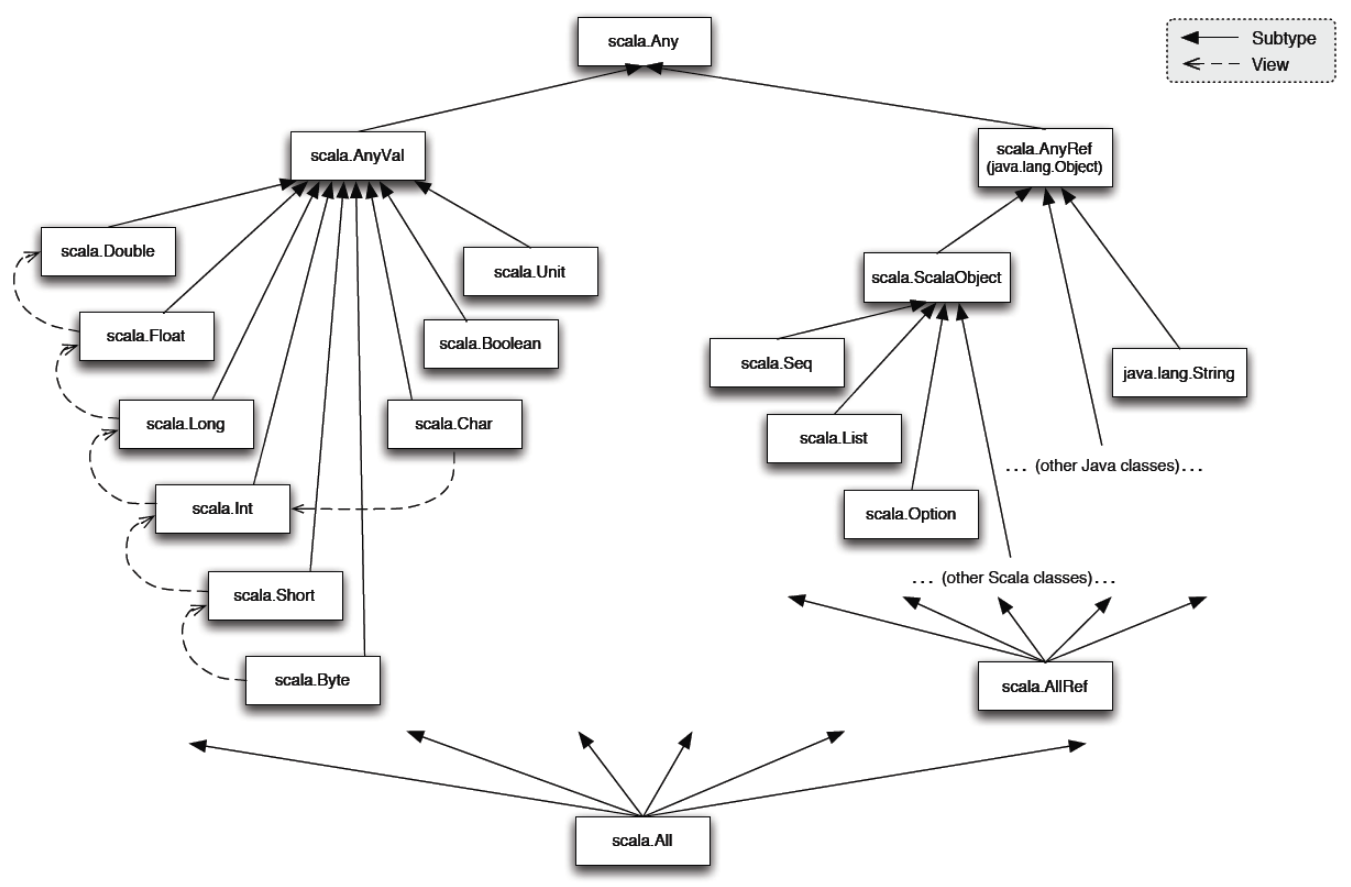
\includegraphics[width=\linewidth]{scala class hierarchy.png}

\subsubsection{Object equality in Scala}

In Scala, you can use \colorbox{yellow}{== to compare objects' contents}.\\
This is different from Java!
\begin{lstlisting}
  > 1 == 2 // remember: numbers are objects!
  res0: Boolean = false
  > List(1,2) == List(1,2)
  res1: Boolean = true
  > 1 == 1.0 // objects of different types!
  res2: Boolean = true
  > ("he"+"llo") == "hello"
  res3: Boolean = true
\end{lstlisting}

So, in Scala,\\
== has been carefully crafted:\\
you get the equality comparison intended in most cases!

Compare with Java:\\
- The same on the primitive types.\\
- On reference/object types,\\
== in Java compares reference/pointer equality\\
== in Scala compares contents equality\\
- \colorbox{yellow}{eq in Scala compares reference/pointer equality}

\subsubsection{Functions}

Define functions in Scala
\begin{lstlisting}
  scala> def sum (xs : List[Int]) : Int =
                xs match {
                  case Nil => 0
                  case x :: ys => x + sum(ys)
                }
  sum: (xs: List[Int])Int
\end{lstlisting}
In Haskell, sum is defined as
\begin{lstlisting}
  sum [] = 0
  sum (x:xs) = x + sum xs
\end{lstlisting}

In Scala, functions\\
- Are \colorbox{yellow}{first-class}\\
- Can be partially applied\\
- Can be higher-order

Functions can be changed (“mutable”)
\begin{lstlisting}
  > var inc = (x:Int) => x+1
  inc : (Int) => Int
  > inc(10)
  res0: Int = 11
  > inc = (x:Int) => {
      x+1000
      println("inc changed")
    }
  inc : (Int) => Int
  > inc(10)
  res1: Int = 1010
  inc changed
\end{lstlisting}

\colorbox{yellow}{foreach}
\begin{lstlisting}
  > List(-10,11,2).foreach((x:Int)=>println(x))
  -10
  11
  2
  > List(-10,11,2).filter((x:Int) => x<0)
  res2: List[Int] = List(-10)
\end{lstlisting}

foreach(f)\\
- is a method, like “map” except that it does not return a value.\\
- applies the argument function to each element of a list.

\colorbox{yellow}{Closures}
\begin{lstlisting}
  var more = 3;
  val addMore = (x : Int) => x + more
  addMore(10) // 13
  more = 1000
  addMore(10) // 1010
\end{lstlisting}
Note: more is an (open) variable wrt addMore.

In Scala, a function body can access variables!\\
Many PLs support closures.\\
- Ruby, Python, JavaScript, …\\
- This, of course, does not imply that this is a good feature …

\colorbox{yellow}{for-comprehension} (cf, list comprehension in Haskell)
\begin{lstlisting}
  scala> for(i <- 1 to 30;
         | j <- List(2,3,5,7);
         | if i % j == 0) yield (i,j)

  res0: scala.collection.immutable.IndexedSeq[(Int, Int)] =
  Vector((2,2), (3,3), (4,2), (5,5), (6,2),
  (6,3), (7,7), (8,2), (9,3), (10,2), (10,5), (12,2),
  (12,3), (14,2), (14,7), (15,3), (15,5), (16,2),
  (18,2), (18,3), (20,2), (20,5), (21,3), (21,7),
  (22,2), (24,2), (24,3), (25,5), (26,2), (27,3),
  (28,2), (28,7), (30,2), (30,3), (30,5))
\end{lstlisting}

%TODO  Chapter 1 of “Programming in Scala" (book on the right) Page & Scala Tutorial for Java Programmers

\chapter{Week 8 - FP in Scala and Recursion in FP}

Scala can do most of what can be done in Haskell.\\
Does not mean that Scala can do it well, though. (Problem with typing ...)

\section{FP in Scala}

\subsection{Recursive functions}

Haskell;
\begin{lstlisting}
  sum [] = 0
  sum (x:xs) = x + sum xs
\end{lstlisting}

Scala;
\begin{lstlisting}
  scala> def sum (xs : List[Int]) : Int =
            xs match {
              case Nil => 0
              case x :: ys => x + sum(ys)
            }
  sum: (xs: List[Int])Int
  scala> sum (List(1,2,3))
  res2: Int = 6
\end{lstlisting}
In Scala, \colorbox{yellow}{recursive function definitions require explicit result types} (Int in the above) as well as \colorbox{yellow}{parameter types}
(List[Int]), which \colorbox{yellow}{are always required}

\colorbox{cyan}{Two styles of typing}:\\
- Church-style: \lstinline[mathescape]?$\lambda$x:A.b? (with domain’s type label)\\
- Curry-style: \lstinline[mathescape]?$\lambda$x.b? (without domain’s type label)

But in Scala, \colorbox{cyan}{more needed}:\\
\lstinline[mathescape]?$\lambda$x:A. (b : B)? - \colorbox{yellow}{labelling both domain and range!}

Domain’s type labelling is needed for sophisticated TTs (e.g., with dependent types)\\
But to label range as well is just unnatural (symptom …?)

\subsection{Polymorphic functions}

In Haskell:
\begin{lstlisting}
  length :: [a] -> Int
\end{lstlisting}
\colorbox{yellow}{Type parameters} in Scala (T in the example below)
\begin{lstlisting}
  scala> def length [T] (xs: List[T]) : Int =
            xs match {
              case Nil => 0
              case x :: ys => length(ys) + 1
            }
  length: [T](xs: List[T])Int
  scala> length (List(1,2,3))
  res3: Int = 3
\end{lstlisting}

In Haskell, no need for type labels:\\
\lstinline?length :: [a]->Int?\\
In Scala, \colorbox{yellow}{both labels needed}:\\
\lstinline?length : [T] (xs:List[T]) Int?

The following is OK in Scala:
\begin{lstlisting}
  scala> length (List(1,List(1)))
  res4: Int = 2
\end{lstlisting}
Why? [1,[1]] would not be well-typed in Haskell, but
its corresponding expression is in Scala:
\begin{lstlisting}
  scala> List(1,List(1))
  res5: List[Any] = List(1,List(1))
\end{lstlisting}
Because: Any is a supertype of both Int and List[Int]!

If A$\leq$B and if a:A, then a:B.\\
So, since Int$\leq$Any and List[Int]$\leq$Any, 1:Any and
List(1):Any, and hence the above.

\colorbox{yellow}{Heterogeneous lists}\\
\begin{lstlisting}
  l = [ 1, [2,3], \x->x ]
\end{lstlisting}
\colorbox{yellow}{Possible in Scala}:\\
l : List[Any]\\
because Int < Any, List[Int] < Any, …\\
(every type is a subtype of Any)

\subsection{Pattern matching}

\colorbox{yellow}{List patterns} in the examples earlier.

For example, the reverse function:\\
In Haskell:
\begin{lstlisting}
  reverse :: [a] -> [a]
  reverse [] = []
  reverse (x:xs) = reverse xs ++ [x]
\end{lstlisting}
In Scala:
\begin{lstlisting}
  def reverse [T] (xs : List[T]) : List[T] =
    xs match {
      case Nil => Nil
      case x::ys => reverse(ys) ::: List(x)
    }
\end{lstlisting}

\colorbox{cyan}{Three colon-signs};\\
\begin{tabular}{c c c}
      & \underline{Haskell} & \underline{Scala} \\
  :   & cons                & typing            \\
  ::  & typing              & cons              \\
  ::: & (++ instead)        & concatenation     \\
\end{tabular}

Other patterns such as \colorbox{yellow}{pair-patterns}:\\
In Haskell:
\begin{lstlisting}
  True && True = True
  _ && _ = False
\end{lstlisting}
In Scala:
\begin{lstlisting}
  def AND (x:Boolean,y:Boolean) : Boolean =
    (x,y) match {
      case (true,true) => true
      case (_,_) => false
    }
\end{lstlisting}

\subsection{Anonymous functions}

Consider the following function in Haskell:\\
\lstinline?odds n = map (\x -> x*2 + 1) [0..n-1]?\\
In Scala, this can be done as\\
\lstinline?def odds (n:Int) = List.range(0,n-1) map ((x:Int) => x*2+1)?\\
Note, besides the \colorbox{yellow}{anonymous function}, the use of List.range(m,n) (in Haskell, this is [m,n-1]).

\subsection{Sequence/list comprehensions}

List comprehension is called \colorbox{yellow}{sequence comprehension} in Scala.

In Haskell, eg, \lstinline?> [x*x | x <- [1..3]]?\\
In Scala (notice “4” here),
\begin{lstlisting}
  scala> for (x<-List.range(1,4)) yield x*x
  res6: List[Int] = List(1,4,9)
\end{lstlisting}
Also, we can have \colorbox{yellow}{nested \& dependent generators}:
\begin{lstlisting}
  scala> for (x<-List.range(1,2))
          yield for (y<-List.range(x,4))
          yield (x,y)
  res7: List[List[(Int,Int)]] = List(List((1,1),(1,2),(1,3)))
\end{lstlisting}

\colorbox{yellow}{List of lists};\\
In Haskell, \lstinline?[ [(x,y) | y <- [x, 3]] | x <- [1] ]?\\
e.g.
\begin{lstlisting}
  qsort [] = []
  qsort (x:xs) =
    qsort smaller ++ [x] ++ qsort larger
    where
      smaller = [a | a <- xs, a <= x]
      larger = [b | b <- xs, b > x]
\end{lstlisting}

In Scala:
\begin{lstlisting}
  def qsort (xs : List[Int]) : List[Int] =
    xs match {
      case Nil => Nil
      case x :: ys =>
        qsort(for (i<-ys if i<=x) yield i)
      ::: List(x)
      ::: qsort(for (j<-ys if j>x) yield j)
    }
\end{lstlisting}

\subsection{more example functions}

\subsubsection{factors}

Haskell:
\begin{lstlisting}
  factors :: Int -> [Int]
  factors n =
    [x | x <- [1..n], n `mod` x == 0]
\end{lstlisting}
Scala:
\begin{lstlisting}
  def factors (n:Int) =
    for (x <- List.range(1,n+1) if n % x == 0)
    yield x
\end{lstlisting}

\subsubsection{Predicate prime and function primes}

Haskell:
\begin{lstlisting}
  prime :: Int -> Bool
  prime n = factors n == [1,n]

  primes :: Int -> [Int]
  primes n = [x | x <- [2..n], prime x]
\end{lstlisting}
Scala:
\begin{lstlisting}
  def prime (n:Int) = factors(n) == List(1,n)
  def primes (n:Int) =
    for (x <- List.range(2,n+1) if prime(x))
    yield x
\end{lstlisting}

\subsubsection{Adjacent pairs and “sorted”}
Haskell:
\begin{lstlisting}
  pairs :: [a] -> [(a,a)]
  pairs xs = zip xs (tail xs)
  sorted :: Ord a => [a] -> Bool
  sorted xs = and [x < y | (x,y) <- pairs xs]
\end{lstlisting}

Scala:
\begin{lstlisting}
  def adj_pairs [T] (xs : List[T]) = xs zip xs.tail
  def and_list (xs:List[Boolean]) : Boolean =
    xs match {
      case Nil => true
      case b::ys => b && and_list(ys)
    }
  def sorted (xs:List[Int]) =
    and_list (for ( (x,y) <- adj_pairs(xs) )
                yield x <= y
              )
\end{lstlisting}

Remember: in Scala, range type-labelling is required
for recursively defined functions.

adj\_pairs/sorted are non-recursive, so no need for
range labelling.

But, and\_list is recursively defined, so needed.

%TODO read Sections 8.1 – 8.6 of “Programming in Scala"

\section{Recursion}

Recursion is the basic looping mechanism in FP.\\
Eg,
\begin{lstlisting}
  factorial :: Int -> Int
  factorial 0 = 1
  factorial n = n * factorial (n-1)
\end{lstlisting}
or
\begin{lstlisting}
  mult :: Int -> Int -> Int
  mult m 0 = 0
  mult m n = m + (mult m (n-1))
\end{lstlisting}

The recursive definition diverges on integers \textless 0
because the base case is never reached:
\begin{lstlisting}
  > factorial (-1)
  <interactive>: out of memory
\end{lstlisting}
Can define factorials as
\begin{lstlisting}
  factorial :: Int->Int
  factorial 0 = 1
  factorial n | n>0 = n * factorial (n-1)
\end{lstlisting}
\begin{lstlisting}
  > factorial (-1)
  *** Exception: ... Non-exhaustive patterns ...
\end{lstlisting}
Or even as
\begin{lstlisting}
  factorial :: Int->Int
  factorial n | n<=0 = 1
  factorial n | n>0 = n * factorial (n-1)
\end{lstlisting}

\subsection{Why is Recursion Useful?}

Cf, loops

Some functions, such as factorial, are \colorbox{pink}{simpler to define}
in terms of other functions (eg, factorial n = product
  [1..n]).

Many functions can \colorbox{pink}{naturally be defined by recursion}.

Properties of functions defined using recursion can be
proved using the simple but powerful mathematical
technique of induction.

\subsection{Recursion on Lists}

\begin{lstlisting}
  product :: [Int] -> Int
  product [] = 1
  product (n:ns) = n * product ns
\end{lstlisting}
product maps the empty list to 1, and any
non-empty list to its head multiplied by the
product of its tail.

The same pattern;
\begin{lstlisting}
  length :: [a] -> Int
  length [] = 0
  length (_:xs) = 1 + length xs
\end{lstlisting}
length maps the empty list to 0, and any
non-empty list to the successor of the
length of its tail.

likewise;
\begin{lstlisting}
  reverse :: [a] -> [a]
  reverse [] = []
  reverse (x:xs) = reverse xs ++ [x]
\end{lstlisting}

reverse maps the empty list to the empty list, and
any non-empty list to the reverse of its tail
appended to its head.

\subsection{Multiple Arguments}

\colorbox{pink}{Functions with more than one argument can also be
  defined using recursion}. For example:

Zipping the elements of two lists:
\begin{lstlisting}
  zip :: [a] -> [b] -> [(a,b)]
  zip [] _ = []
  zip _ [] = []
  zip (x:xs) (y:ys) = (x,y) : zip xs ys
\end{lstlisting}

Remove the first n elements from a list:
\begin{lstlisting}
  drop :: Int -> [a] -> [a]
  drop 0 xs = xs
  drop n [] = []
  drop n (_:xs) = drop (n-1) xs
\end{lstlisting}

Appending two lists:
\begin{lstlisting}
  (++) :: [a] -> [a] -> [a]
  [] ++ ys = ys
  (x:xs) ++ ys = x : (xs ++ ys)
\end{lstlisting}

\subsection{Quicksort}

The quicksort algorithm for sorting a list of integers can be
specified by the following two rules:\\
1. The empty list is already sorted;\\
2. Non-empty lists can be sorted by sorting the tail values
$\leq$ the head, sorting the tail values \textgreater the head, and then
appending the resulting lists on either side of the head
value.

Using recursion, this specification can be translated directly
into an implementation:
\begin{lstlisting}
  qsort :: [Int] -> [Int]
  qsort [] = []
  qsort (x:xs) =
  qsort smaller ++ [x] ++ qsort larger
    where
      smaller = [a | a <- xs, a <= x]
      larger = [b | b <- xs, b > x]
\end{lstlisting}

This is probably the simplest implementation of quicksort in any programming language!

\subsection{Mutual recursion}

\begin{lstlisting}
  even :: Int -> Bool
  even 0 = True
  even n = odd (n-1)

  odd :: Int -> Bool
  odd 0 = False
  odd n = even (n-1)
\end{lstlisting}

Functions selecting elements at even/odd
positions in a list:
\begin{lstlisting}
  evens :: [a] -> [a]
  evens [] = []
  evens (x:xs) = x : odds xs

  odds :: [a] -> [a]
  odds [] = []
  odds (_:xs) = evens xs
\end{lstlisting}

Advice on writing recursive functions\\
- they become simpler, more natural, and easier with practice

\colorbox{cyan}{Five-step process};\\
- Define the type\\
- Enumerate the cases\\
- Define the simple/base cases\\
- Define the other/step cases\\
- Generalise and/or simplify

%TODO read Chapter 7 (of the Haskell book)

\chapter{Week 9 - Lazy Evaluation and Advanced Topics}

\section{Lazy Evaluation}

Avoids doing unnecessary evaluation\\
Allows programs to be more modular\\
Allows one to program with infinite lists

No other popular FP lang uses lazy evaluation

\subsection{Expression evaluation}

Expressions are evaluated or reduced by\\
- successively expanding definitions (or doing $\beta$-reduction) by
evaluating/\colorbox{yellow}{reducing redexes} (reducible expressions)\\
- until no further simplification is possible\\
- Evaluation order\\
- There can be different orders in evaluating expressions\\
- In “well-behaving” (pure) FP languages like Haskell, any two
different (but terminating) reductions of the same expression end
with the same result no matter it is evaluated in which order. (But
different in an impure FP lang!)\\
(Technical jargon: Church-Rosser property.)

\colorbox{cyan}{Several kinds of redexes} (reducible expressions);\\
$\delta$-redex:\\
- Reducing a $\delta$-redex is to expand a definition.\\
- Example: square(7) -> 7 * 7\\
$\beta$-redex:\\
- \lstinline?(\x.b[x])(a) -> b[x]?\\
- Example: if \lstinline?+ = \xy. ...? then reducing 3+4 involves $\beta$-reduction

Different orders of evaluation example\\
Eg, given\\
\lstinline?square n = n * n?\\
\lstinline?square(3+4)? can be evaluated using the following sequence of reductions:
\begin{lstlisting}
  square (3+4) = square 7
  = 7 * 7
  = 49
\end{lstlisting}
The above is not the only possible reduction sequence.\\
Another is:
\begin{lstlisting}
  square (3+4) = (3+4) * (3+4)
  = 7 * (3+4)
  = 7 * 7
  = 49
\end{lstlisting}

Different orders of evaluations in impure FP languages may give different results!\\
Example:\\
\begin{lstlisting}
  var n = 0;
  var m = n + (n = 1) [2nd = is assignment!]
\end{lstlisting}
Evaluate n + (n = 1):\\
(1) n + \underline{(n = 1)} -> n+1 -> 1+1 -> 2\\
(2) \underline{n} + (n = 1) -> 0+(n=1) -> 0+1 -> 1

\subsubsection{Church-Rosser property}

Theorem proved by Church \& Rosser in 1936

\colorbox{yellow}{If e evaluates to e1 and e2, then there exists an expression
  e’ such that e1 and e2 both evaluates to e’}.

\begin{figure}[H]
  \centering
  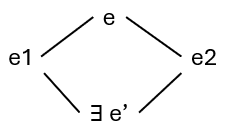
\includegraphics[width=.3\linewidth]{Church-Rosser property.png}
\end{figure}


Hence, we have\\
- The final result of evaluating an expression is independent
on the evaluation order.\\
- In Haskell, two different (but terminating) ways of
evaluating the same expression will always give the same
final result.

\subsubsection{Evaluation/reduction strategies}

Possibly more than one redex (reducible expression)
in an expression – which one to eval/reduce?

Two common strategies\\
Innermost reduction;\\
- Always selecting an innermost redex to reduce\\
- Call by value\\
Outermost reduction\\
- Always selecting an outermost redex to reduce\\
- Call by name\\

How do the two strategies compare? Termination\\
Consider a non-terminating expression $\bot$ = tail $\bot$\\
Eg, evaluating fst(1,$\bot$)\\
- Innermost: fst(1,$\bot$) = fst(1,tail $\bot$) = fst(1,tail (tail$\bot$)) = ...\\
- Outermost: fst(1,$\bot$) = 1\\
Hence\\
- Outermost reduction may give a result when the innermost
reduction fails to terminate.\\
- Also, for any expression, if there exists any reduction sequence
that terminates, then the outermost reduction also terminates and
gives the same result.

Number of reduction steps - Efficiency in evaluation\\
- Outermost reduction may require more steps than the innermost reduction\\
Eg, consider square(3+4)\\
- 3+4 is evaluated twice in outermost reduction but only once in innermost one

How to solve the problem? Sharing\\
using pointers to indicate sharing of expressions during evaluation\\
square(3+4) = \textperiodcentered * \textperiodcentered (where \textperiodcentered is 3+4)\\
= \textperiodcentered * \textperiodcentered (where \textperiodcentered is 7)\\
= 49


\colorbox{yellow}{Lazy evaluation = outermost reduction + sharing}\\
Lazy evaluation does not require more reduction steps than
the innermost evaluation.

Example with (potentially) infinite list
\begin{lstlisting}
  ones : [Int]
  ones = 1 : ones
\end{lstlisting}
Evaluating head ones\\
- Innermost: head ones = head (1:ones) = head (1:(1:ones)) = ...\\
- Lazy evaluation: head ones = head (1:ones) = 1

The Slogan:\\
Using lazy evaluation, expressions are only evaluated as much as
required to produce the final result.\\
(cf, the word “potential” above - an infinite list is only evaluated as
much as required in the context in which it is used.)

An extra evaluation strategy in Haskell\\
No evaluation/reduction under lambda\\
eg, \lstinline?(\x -> 1+2+x) 3 = 1+2+3 = 3+3 = 6?\\
Not: \lstinline?(\x -> 1+2+x) 3 = (\x -> 3+x) 3 = 3+3 = 6?\\
In Haskell. \colorbox{yellow}{Lambda-expressions are viewed as values} (normal forms – not to be further evaluated.)

\section{Advanced topics}

\subsection{Parallel programming with FP}

More important in recent years (fast hardware development)

Software is lacking behind ...\\
FP is becoming more attractive and important since FP
programs, especially pure ones, are easy to be executed in
parallel.

Currently a hot research topic (eg, MIT, ...)

\subsection{Typing in FP}

- Types (purpose, etc)
- Church-style v.s. Curry-style typings
- Polymorphic typing (today)
- Dependent typing (today)
- Problems in Multiparadigm PLs such as Scala

\subsection{Let-polymorphism}

Haskell is (and many other FP languages are) based
on this.

\begin{figure}[H]
  \centering
  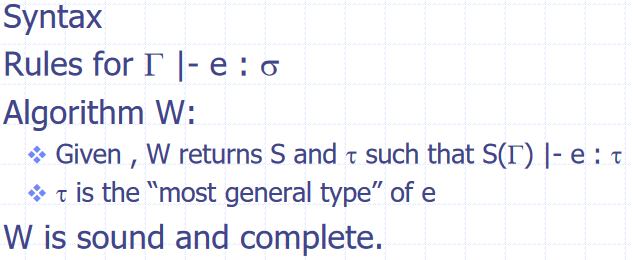
\includegraphics[width=.4\linewidth]{let poly.png}
\end{figure}

\subsection{Dependent types}

Example\\
- Head of a list\\
- Haskell:\\
\lstinline?head :: [a] -> a?, where “head []” raises an exception.\\
\lstinline?safeHead :: a->[a]->a?, where safeHead v [] = v.\\
- With dependent types:\\
\lstinline[mathescape]?Head :: $\forall$n:Nat. Vect(a,n+1)->a?
Head [] is then ill-typed (statically).

\subsection{Heterogeneous Lists}

Several things allow heterogeneous lists;\\
- Subtyping with a top type (e.g., Scala with “Any”)\\
- Type universes in dependent type theories

Type universe: “type of types”.\\
- E.g. A→B : U if A : U and B : U\\
- Then, the type List($\Sigma$A:U.A) consists of lists of pairs:\\
\lstinline?[ (A,a), (B,b), (C,c), ... ]?\\
which is essentially\\
\lstinline?[ a, b, c, ...]?\\
with a/b/c of possibly different types!

\subsection{Type theories}

There are Dependent type theories

Types \& logic!\\
- A x B = A $\wedge$ B\\
- $\forall$x:A.B(x) = $\Pi$x:A.B(x)

So, in the same language, we have Programs + Logic\\
This is only available in dependent type theories (not in other languages).

Typing in multiparadigm PLs;\\
- Unclear how to get a complete/correct typing system, if it
exists\\
- there are problems, eg, with side-effects\\
eg, Scala’s “closure” whose application value depends on the value of
the free variables in its expressions/bodies.

\chapter{Questions \& Answers}

\section{safetail}

Consider a function safetail that behaves in the same way as tail, except
that safetail maps the empty list to the empty list, whereas tail gives an
error in this case. Define safetail using:\\
1. a conditional expression;\\
2. pattern matching;\\
3. guarded equations.\\
(Hint: the library function \lstinline?null :: [a] -> Bool? can be used to test if a
list is empty.)

\begin{lstlisting}
  safetail1 xs = if null xs
                 then []
                 else tail xs
\end{lstlisting}
\begin{lstlisting}
  safetail [] = []
  safetail xs = tail xs
\end{lstlisting}
\begin{lstlisting}
  safetail xs | null xs = []
               | otherwise = tail xs
\end{lstlisting}

\section{pyths}

A triple $(x,y,z)$ of positive integers is called pythagorean if $x^2 + y^2 = z^2$. Using
a list comprehension, define a function
\lstinline?pyths :: Int -> [(Int,Int,Int)]?
that maps an integer n to all pythagorean triples $(a_1, a_2, a_3)$ with components
$a_i$ in \lstinline?[1..n]?.

It's\\
$pyths = \{(x, y, z)\ |\ x, y, z \in \{1..n\},\ x^2 + y^2 = z^2\}$\\
so we have
\begin{lstlisting}
  pyths :: Int -> [(Int, Int, Int)]
  pyths n =
    [ (x, y, z) | x <- [1 .. n]
                , y <- [1 .. n]
                , z <- [1 .. n]
                , x * x + y * y == z * z ]
\end{lstlisting}

\section{map \& filter}

Express the comprehension \lstinline?[ f x | x <- xs, p x ]? using the functions \lstinline?map?
and \lstinline?filter?

\begin{lstlisting}
  myFunc f p xs = map f (filter p xs)
\end{lstlisting}

\section{balanced}

Consider the following type of binary trees of integers:
\begin{lstlisting}
  data Tree = Leaf Int | Node Tree Tree
              deriving (Show)
\end{lstlisting}
Such a tree is balanced if the number of leaves in the left and right subtrees
of every node differs by at most one, with leaves themselves being trivially
balanced.

Define a function \lstinline?balanced :: Tree -> Bool? that decides whether a tree
is balanced. (Hint: first define a function that returns the number of leaves of
a tree.)

Firstly, let’s look at some example values of type \lstinline?Tree?:
\begin{lstlisting}
  ex1 :: Tree
  ex1 = Leaf 0

  ex2 :: Tree
  ex2 = Node (Leaf 0) (Leaf 2)

  ex3 :: Tree
  ex3 = Node (Leaf 1)
              (Node (Leaf 1)
                    (Node (Leaf 3) (Leaf 4)))
\end{lstlisting}
This gives us a bit of an intuition for the shape of our data type. Unsurprisingly,
it resembles a tree.

\begin{lstlisting}
  numLeaves :: Tree -> Int
  numLeaves (Leaf n) = 1
  numLeaves (Node l r) = numLeaves l + numLeaves r

  balanced :: Tree -> Bool
  balanced (Leaf n) = True
  balanced (Node l r) = abs (numLeaves l - numLeaves r) <= 1
                        && balanced l
                        && balanced r
 \end{lstlisting}

\section{insertionSort}

To answer this question, you should first define an insert function
and then use it to define a function for insertion sort.

Define a function \lstinline?insert :: Int->[Int]->[Int]? so that \lstinline?insert x xs?
inserts x to the list xs in such a way that x is bigger than those
elements before it and smaller than or equal to the element that
follows it. For instance,\\
\begin{lstlisting}
  > insert 5 [1,2,4,8,3,6]
  [1,2,4,5,8,3,6]
\end{lstlisting}

Use insert to define a function \lstinline?insertionSort :: [Int]->[Int]?
for insertion sort.

\begin{lstlisting}
iSort :: [Int] -> [Int]
iSort [] = []
iSort (x:xs) = ins x (iSort xs)

ins :: Int -> [Int] -> [Int]
ins x [] = [x]
ins x (y: ys)
      | x <= y = x : (y:ys)
      | otherwise = y : ins x ys
\end{lstlisting}

\section{fib}

The Fibonacci function \textit{Fib} is defined as follows: for any non-negative
integer $n$,
\begin{equation*}
  Fib(n) =
  \begin{cases}
    n,                      & \text{if $n = 0$ or $n = 1$} \\
    Fib(n - 1) + Fib(n - 2) & \text{if $n \geq 2$}         \\
  \end{cases}
\end{equation*}
Using recursion directly, define a function \lstinline?fib :: Int -> Integer?
in Haskell to implement the Fibonacci function.

\begin{lstlisting}
  fib :: Int -> Integer
  fib 0 = 0
  fib 1 = 1
  fib n
      | n > 1 = fib (n-1) + fib (n-2)
      | otherwise = error "negative input to fib"
\end{lstlisting}

Write a non-recursive method in Java to implement the Fibonacci
function.

\begin{lstlisting}
  public fib(int n) {
    if (n <= -1) then return -1;
    if (n <= 2) then return n;

    int fold = 1;
    int fold2 = 1;
    int fnew = 1;

    for (int i=3; i<=n; i++){
      fnew = fold + fold2;
      fold2 = fold;
      fold = fnew;
    }

    return fnew;
  }
\end{lstlisting}

\end{document}